\documentclass[11pt,fleqn]{book}
\usepackage[french]{babel}
\selectlanguage{french}
\usepackage[T1]{fontenc}
\usepackage[utf8]{inputenc}

\newcommand{\graphe}[2]{\includegraphics[width=#1]{#2}}%
\newcommand{\tabref}[1]{Tab.~\ref{#1}}
\newcommand{\figref}[1]{Fig.~\ref{#1}}
\newcommand{\defref}[1]{Def.~\ref{#1}}
\newcommand{\chapref}[1]{Chap.~\ref{#1}}
\newcommand{\secref}[1]{\S\ref{#1}}
\def\cad{c.-à-d.} % les defs du style du poly
%%%%%%%%%%%%%%%%%%%%%%%%%%%%%%%%%%%%%%%%%
% The Legrand Orange Book
% Structural Definitions File
% Version 2.1 (26/09/2018)
%
% Original author:
% Mathias Legrand (legrand.mathias@gmail.com) with modifications by:
% Vel (vel@latextemplates.com)
% 
% This file was downloaded from:
% http://www.LaTeXTemplates.com
%
% License:
% CC BY-NC-SA 3.0 (http://creativecommons.org/licenses/by-nc-sa/3.0/)
%
%%%%%%%%%%%%%%%%%%%%%%%%%%%%%%%%%%%%%%%%%

%----------------------------------------------------------------------------------------
%	VARIOUS REQUIRED PACKAGES AND CONFIGURATIONS
%----------------------------------------------------------------------------------------

\usepackage{graphicx} % Required for including pictures
\graphicspath{{./poly/Pictures/}} % Specifies the directory where pictures are stored

\usepackage{lipsum} % Inserts dummy text

\usepackage{tikz} % Required for drawing custom shapes


\usepackage{enumitem} % Customize lists
\setlist{nolistsep} % Reduce spacing between bullet points and numbered lists

\usepackage{booktabs} % Required for nicer horizontal rules in tables

\usepackage{xcolor} % Required for specifying colors by name
\definecolor{ocre}{RGB}{243,102,25} % Define the orange color used for highlighting throughout the book

%----------------------------------------------------------------------------------------
%	MARGINS
%----------------------------------------------------------------------------------------

\usepackage{geometry} % Required for adjusting page dimensions and margins

\geometry{
	paper=a4paper, % Paper size, change to letterpaper for US letter size
	top=3cm, % Top margin
	bottom=3cm, % Bottom margin
	left=3cm, % Left margin
	right=3cm, % Right margin
	headheight=14pt, % Header height
	footskip=1.4cm, % Space from the bottom margin to the baseline of the footer
	headsep=10pt, % Space from the top margin to the baseline of the header
	%showframe, % Uncomment to show how the type block is set on the page
}

%----------------------------------------------------------------------------------------
%	FONTS
%----------------------------------------------------------------------------------------

\usepackage{avant} % Use the Avantgarde font for headings
%\usepackage{times} % Use the Times font for headings
\usepackage{mathptmx} % Use the Adobe Times Roman as the default text font together with math symbols from the Sym­bol, Chancery and Com­puter Modern fonts

\usepackage{microtype} % Slightly tweak font spacing for aesthetics

%----------------------------------------------------------------------------------------
%	BIBLIOGRAPHY AND INDEX
%----------------------------------------------------------------------------------------
\usepackage{csquotes}
\usepackage[style=numeric,citestyle=numeric,sorting=nyt,sortcites=true,autopunct=true,autolang=hyphen,hyperref=true,abbreviate=false,backref=true,backend=biber]{biblatex}
\addbibresource{bibliography.bib} % BibTeX bibliography file
\defbibheading{bibempty}{}

\usepackage{calc} % For simpler calculation - used for spacing the index letter headings correctly
\usepackage{makeidx} % Required to make an index
\makeindex % Tells LaTeX to create the files required for indexing

%----------------------------------------------------------------------------------------
%	MAIN TABLE OF CONTENTS
%----------------------------------------------------------------------------------------

\usepackage{titletoc} % Required for manipulating the table of contents

\contentsmargin{0cm} % Removes the default margin

% Part text styling (this is mostly taken care of in the PART HEADINGS section of this file)
\titlecontents{part}
	[0cm] % Left indentation
	{\addvspace{20pt}\bfseries} % Spacing and font options for parts
	{}
	{}
	{}

% Chapter text styling
\titlecontents{chapter}
	[1.25cm] % Left indentation
	{\addvspace{12pt}\large\sffamily\bfseries} % Spacing and font options for chapters
	{\color{ocre!60}\contentslabel[\Large\thecontentslabel]{1.25cm}\color{ocre}} % Formatting of numbered sections of this type
	{\color{ocre}} % Formatting of numberless sections of this type
	{\color{ocre!60}\normalsize\;\titlerule*[.5pc]{.}\;\thecontentspage} % Formatting of the filler to the right of the heading and the page number

% Section text styling
\titlecontents{section}
	[1.25cm] % Left indentation
	{\addvspace{3pt}\sffamily\bfseries} % Spacing and font options for sections
	{\contentslabel[\thecontentslabel]{1.25cm}} % Formatting of numbered sections of this type
	{} % Formatting of numberless sections of this type
	{\hfill\color{black}\thecontentspage} % Formatting of the filler to the right of the heading and the page number

% Subsection text styling
\titlecontents{subsection}
	[1.25cm] % Left indentation
	{\addvspace{1pt}\sffamily\small} % Spacing and font options for subsections
	{\contentslabel[\thecontentslabel]{1.25cm}} % Formatting of numbered sections of this type
	{} % Formatting of numberless sections of this type
	{\ \titlerule*[.5pc]{.}\;\thecontentspage} % Formatting of the filler to the right of the heading and the page number

% Figure text styling
\titlecontents{figure}
	[1.25cm] % Left indentation
	{\addvspace{1pt}\sffamily\small} % Spacing and font options for figures
	{\thecontentslabel\hspace*{1em}} % Formatting of numbered sections of this type
	{} % Formatting of numberless sections of this type
	{\ \titlerule*[.5pc]{.}\;\thecontentspage} % Formatting of the filler to the right of the heading and the page number

% Table text styling
\titlecontents{table}
	[1.25cm] % Left indentation
	{\addvspace{1pt}\sffamily\small} % Spacing and font options for tables
	{\thecontentslabel\hspace*{1em}} % Formatting of numbered sections of this type
	{} % Formatting of numberless sections of this type
	{\ \titlerule*[.5pc]{.}\;\thecontentspage} % Formatting of the filler to the right of the heading and the page number

%----------------------------------------------------------------------------------------
%	MINI TABLE OF CONTENTS IN PART HEADS
%----------------------------------------------------------------------------------------

% Chapter text styling
\titlecontents{lchapter}
	[0em] % Left indentation
	{\addvspace{15pt}\large\sffamily\bfseries} % Spacing and font options for chapters
	{\color{ocre}\contentslabel[\Large\thecontentslabel]{1.25cm}\color{ocre}} % Chapter number
	{}  
	{\color{ocre}\normalsize\sffamily\bfseries\;\titlerule*[.5pc]{.}\;\thecontentspage} % Page number

% Section text styling
\titlecontents{lsection}
	[0em] % Left indentation
	{\sffamily\small} % Spacing and font options for sections
	{\contentslabel[\thecontentslabel]{1.25cm}} % Section number
	{}
	{}

% Subsection text styling (note these aren't shown by default, display them by searchings this file for tocdepth and reading the commented text)
\titlecontents{lsubsection}
	[.5em] % Left indentation
	{\sffamily\footnotesize} % Spacing and font options for subsections
	{\contentslabel[\thecontentslabel]{1.25cm}}
	{}
	{}

%----------------------------------------------------------------------------------------
%	HEADERS AND FOOTERS
%----------------------------------------------------------------------------------------

\usepackage{fancyhdr} % Required for header and footer configuration

\pagestyle{fancy} % Enable the custom headers and footers

\renewcommand{\chaptermark}[1]{\markboth{\sffamily\normalsize\bfseries\chaptername\ \thechapter.\ #1}{}} % Styling for the current chapter in the header
\renewcommand{\sectionmark}[1]{\markright{\sffamily\normalsize\thesection\hspace{5pt}#1}{}} % Styling for the current section in the header

\fancyhf{} % Clear default headers and footers
\fancyhead[LE,RO]{\sffamily\normalsize\thepage} % Styling for the page number in the header
\fancyhead[LO]{\rightmark} % Print the nearest section name on the left side of odd pages
\fancyhead[RE]{\leftmark} % Print the current chapter name on the right side of even pages
%\fancyfoot[C]{\thepage} % Uncomment to include a footer

\renewcommand{\headrulewidth}{0.5pt} % Thickness of the rule under the header

\fancypagestyle{plain}{% Style for when a plain pagestyle is specified
	\fancyhead{}\renewcommand{\headrulewidth}{0pt}%
}

% Removes the header from odd empty pages at the end of chapters
\makeatletter
\renewcommand{\cleardoublepage}{
\clearpage\ifodd\c@page\else
\hbox{}
\vspace*{\fill}
\thispagestyle{empty}
\newpage
\fi}

%----------------------------------------------------------------------------------------
%	THEOREM STYLES
%----------------------------------------------------------------------------------------

\usepackage{amsmath,amsfonts,amssymb,amsthm} % For math equations, theorems, symbols, etc

\newcommand{\intoo}[2]{\mathopen{]}#1\,;#2\mathclose{[}}
\newcommand{\ud}{\mathop{\mathrm{{}d}}\mathopen{}}
\newcommand{\intff}[2]{\mathopen{[}#1\,;#2\mathclose{]}}
\renewcommand{\qedsymbol}{$\blacksquare$}
\newtheorem{notation}{Notation}[chapter]

% Boxed/framed environments
\newtheoremstyle{ocrenumbox}% Theorem style name
{0pt}% Space above
{0pt}% Space below
{\normalfont}% Body font
{}% Indent amount
{\small\bf\sffamily\color{ocre}}% Theorem head font
{\;}% Punctuation after theorem head
{0.25em}% Space after theorem head
{\small\sffamily\color{ocre}\thmname{#1}\nobreakspace\thmnumber{\@ifnotempty{#1}{}\@upn{#2}}% Theorem text (e.g. Theorem 2.1)
\thmnote{\nobreakspace\the\thm@notefont\sffamily\bfseries\color{black}---\nobreakspace#3.}} % Optional theorem note

\newtheoremstyle{blacknumex}% Theorem style name
{5pt}% Space above
{5pt}% Space below
{\normalfont}% Body font
{} % Indent amount
{\small\bf\sffamily}% Theorem head font
{\;}% Punctuation after theorem head
{0.25em}% Space after theorem head
{\small\sffamily{\tiny\ensuremath{\blacksquare}}\nobreakspace\thmname{#1}\nobreakspace\thmnumber{\@ifnotempty{#1}{}\@upn{#2}}% Theorem text (e.g. Theorem 2.1)
\thmnote{\nobreakspace\the\thm@notefont\sffamily\bfseries---\nobreakspace#3.}}% Optional theorem note

\newtheoremstyle{blacknumbox} % Theorem style name
{0pt}% Space above
{0pt}% Space below
{\normalfont}% Body font
{}% Indent amount
{\small\bf\sffamily}% Theorem head font
{\;}% Punctuation after theorem head
{0.25em}% Space after theorem head
{\small\sffamily\thmname{#1}\nobreakspace\thmnumber{\@ifnotempty{#1}{}\@upn{#2}}% Theorem text (e.g. Theorem 2.1)
\thmnote{\nobreakspace\the\thm@notefont\sffamily\bfseries---\nobreakspace#3.}}% Optional theorem note

% Non-boxed/non-framed environments
\newtheoremstyle{ocrenum}% Theorem style name
{5pt}% Space above
{5pt}% Space below
{\normalfont}% Body font
{}% Indent amount
{\small\bf\sffamily\color{ocre}}% Theorem head font
{\;}% Punctuation after theorem head
{0.25em}% Space after theorem head
{\small\sffamily\color{ocre}\thmname{#1}\nobreakspace\thmnumber{\@ifnotempty{#1}{}\@upn{#2}}% Theorem text (e.g. Theorem 2.1)
\thmnote{\nobreakspace\the\thm@notefont\sffamily\bfseries\color{black}---\nobreakspace#3.}} % Optional theorem note
\makeatother

% Defines the theorem text style for each type of theorem to one of the three styles above
\newcounter{dummy} 
\numberwithin{dummy}{section}
\theoremstyle{ocrenumbox}
\newtheorem{theoremeT}[dummy]{Theorème}
\newtheorem{probleme}{Problème}[chapter]
\newtheorem{exercisseT}{Exercisse}[chapter]
\theoremstyle{blacknumex}
\newtheorem{exempleT}{Exemple}[chapter]
\theoremstyle{blacknumbox}
\newtheorem{vocabulary}{Vocabulary}[chapter]
\newtheorem{definitionT}{Definition}[section]
\newtheorem{corollaryT}[dummy]{Corollary}
\theoremstyle{ocrenum}
\newtheorem{proposition}[dummy]{Proposition}

%----------------------------------------------------------------------------------------
%	DEFINITION OF COLORED BOXES
%----------------------------------------------------------------------------------------

\RequirePackage[framemethod=default]{mdframed} % Required for creating the theorem, definition, exercise and corollary boxes

% Theorem box
\newmdenv[skipabove=7pt,
skipbelow=7pt,
backgroundcolor=black!5,
linecolor=ocre,
innerleftmargin=5pt,
innerrightmargin=5pt,
innertopmargin=5pt,
leftmargin=0cm,
rightmargin=0cm,
innerbottommargin=5pt]{tBox}

% Exercise box	  
\newmdenv[skipabove=7pt,
skipbelow=7pt,
rightline=false,
leftline=true,
topline=false,
bottomline=false,
backgroundcolor=ocre!10,
linecolor=ocre,
innerleftmargin=5pt,
innerrightmargin=5pt,
innertopmargin=5pt,
innerbottommargin=5pt,
leftmargin=0cm,
rightmargin=0cm,
linewidth=4pt]{eBox}	

% Definition box
\newmdenv[skipabove=7pt,
skipbelow=7pt,
rightline=false,
leftline=true,
topline=false,
bottomline=false,
linecolor=ocre,
innerleftmargin=5pt,
innerrightmargin=5pt,
innertopmargin=0pt,
leftmargin=0cm,
rightmargin=0cm,
linewidth=4pt,
innerbottommargin=0pt]{dBox}	

% Corollary box
\newmdenv[skipabove=7pt,
skipbelow=7pt,
rightline=false,
leftline=true,
topline=false,
bottomline=false,
linecolor=gray,
backgroundcolor=black!5,
innerleftmargin=5pt,
innerrightmargin=5pt,
innertopmargin=5pt,
leftmargin=0cm,
rightmargin=0cm,
linewidth=4pt,
innerbottommargin=5pt]{cBox}

% Creates an environment for each type of theorem and assigns it a theorem text style from the "Theorem Styles" section above and a colored box from above
\newenvironment{theoreme}{\begin{tBox}\begin{theoremeT}}{\end{theoremeT}\end{tBox}}
\newenvironment{exercise}{\begin{eBox}\begin{exerciseT}}{\hfill{\color{ocre}\tiny\ensuremath{\blacksquare}}\end{exerciseT}\end{eBox}}				  
\newenvironment{definition}{\begin{eBox}\begin{definitionT}}{\end{definitionT}\end{eBox}}	
\newenvironment{exemple}{\begin{exempleT}}{\hfill{\tiny\ensuremath{\blacksquare}}\end{exempleT}}		
\newenvironment{corollary}{\begin{cBox}\begin{corollaryT}}{\end{corollaryT}\end{cBox}}	

%----------------------------------------------------------------------------------------
%	REMARK ENVIRONMENT
%----------------------------------------------------------------------------------------

\newenvironment{remarque}{\par\vspace{10pt}\small % Vertical white space above the remark and smaller font size
\begin{list}{}{
\leftmargin=35pt % Indentation on the left
\rightmargin=25pt}\item\ignorespaces % Indentation on the right
\makebox[-2.5pt]{\begin{tikzpicture}[overlay]
\node[draw=ocre!60,line width=1pt,circle,fill=ocre!25,font=\sffamily\bfseries,inner sep=2pt,outer sep=0pt] at (-15pt,0pt){\textcolor{ocre}{R}};\end{tikzpicture}} % Orange R in a circle
\advance\baselineskip -1pt}{\end{list}\vskip5pt} % Tighter line spacing and white space after remark

%----------------------------------------------------------------------------------------
%	SECTION NUMBERING IN THE MARGIN
%----------------------------------------------------------------------------------------

\makeatletter
\renewcommand{\@seccntformat}[1]{\llap{\textcolor{ocre}{\csname the#1\endcsname}\hspace{1em}}}                    
\renewcommand{\section}{\@startsection{section}{1}{\z@}
{-4ex \@plus -1ex \@minus -.4ex}
{1ex \@plus.2ex }
{\normalfont\large\sffamily\bfseries}}
\renewcommand{\subsection}{\@startsection {subsection}{2}{\z@}
{-3ex \@plus -0.1ex \@minus -.4ex}
{0.5ex \@plus.2ex }
{\normalfont\sffamily\bfseries}}
\renewcommand{\subsubsection}{\@startsection {subsubsection}{3}{\z@}
{-2ex \@plus -0.1ex \@minus -.2ex}
{.2ex \@plus.2ex }
{\normalfont\small\sffamily\bfseries}}                        
\renewcommand\paragraph{\@startsection{paragraph}{4}{\z@}
{-2ex \@plus-.2ex \@minus .2ex}
{.1ex}
{\normalfont\small\sffamily\bfseries}}

%----------------------------------------------------------------------------------------
%	PART HEADINGS
%----------------------------------------------------------------------------------------

% Numbered part in the table of contents
\newcommand{\@mypartnumtocformat}[2]{%
	\setlength\fboxsep{0pt}%
	\noindent\colorbox{ocre!20}{\strut\parbox[c][.7cm]{\ecart}{\color{ocre!70}\Large\sffamily\bfseries\centering#1}}\hskip\esp\colorbox{ocre!40}{\strut\parbox[c][.7cm]{\linewidth-\ecart-\esp}{\Large\sffamily\centering#2}}%
}

% Unnumbered part in the table of contents
\newcommand{\@myparttocformat}[1]{%
	\setlength\fboxsep{0pt}%
	\noindent\colorbox{ocre!40}{\strut\parbox[c][.7cm]{\linewidth}{\Large\sffamily\centering#1}}%
}

\newlength\esp
\setlength\esp{4pt}
\newlength\ecart
\setlength\ecart{1.2cm-\esp}
\newcommand{\thepartimage}{}%
\newcommand{\partimage}[1]{\renewcommand{\thepartimage}{#1}}%
\def\@part[#1]#2{%
\ifnum \c@secnumdepth >-2\relax%
\refstepcounter{part}%
\addcontentsline{toc}{part}{\texorpdfstring{\protect\@mypartnumtocformat{\thepart}{#1}}{\partname~\thepart\ ---\ #1}}
\else%
\addcontentsline{toc}{part}{\texorpdfstring{\protect\@myparttocformat{#1}}{#1}}%
\fi%
\startcontents%
\markboth{}{}%
{\thispagestyle{empty}%
\begin{tikzpicture}[remember picture,overlay]%
\node at (current page.north west){\begin{tikzpicture}[remember picture,overlay]%	
\fill[ocre!20](0cm,0cm) rectangle (\paperwidth,-\paperheight);
\node[anchor=north] at (4cm,-3.25cm){\color{ocre!40}\fontsize{220}{100}\sffamily\bfseries\thepart}; 
\node[anchor=south east] at (\paperwidth-1cm,-\paperheight+1cm){\parbox[t][][t]{8.5cm}{
\printcontents{l}{0}{\setcounter{tocdepth}{1}}% The depth to which the Part mini table of contents displays headings; 0 for chapters only, 1 for chapters and sections and 2 for chapters, sections and subsections
}};
\node[anchor=north east] at (\paperwidth-1.5cm,-3.25cm){\parbox[t][][t]{15cm}{\strut\raggedleft\color{white}\fontsize{30}{30}\sffamily\bfseries#2}};
\end{tikzpicture}};
\end{tikzpicture}}%
\@endpart}
\def\@spart#1{%
\startcontents%
\phantomsection
{\thispagestyle{empty}%
\begin{tikzpicture}[remember picture,overlay]%
\node at (current page.north west){\begin{tikzpicture}[remember picture,overlay]%	
\fill[ocre!20](0cm,0cm) rectangle (\paperwidth,-\paperheight);
\node[anchor=north east] at (\paperwidth-1.5cm,-3.25cm){\parbox[t][][t]{15cm}{\strut\raggedleft\color{white}\fontsize{30}{30}\sffamily\bfseries#1}};
\end{tikzpicture}};
\end{tikzpicture}}
\addcontentsline{toc}{part}{\texorpdfstring{%
\setlength\fboxsep{0pt}%
\noindent\protect\colorbox{ocre!40}{\strut\protect\parbox[c][.7cm]{\linewidth}{\Large\sffamily\protect\centering #1\quad\mbox{}}}}{#1}}%
\@endpart}
\def\@endpart{\vfil\newpage
\if@twoside
\if@openright
\null
\thispagestyle{empty}%
\newpage
\fi
\fi
\if@tempswa
\twocolumn
\fi}

%----------------------------------------------------------------------------------------
%	CHAPTER HEADINGS
%----------------------------------------------------------------------------------------

% A switch to conditionally include a picture, implemented by Christian Hupfer
\newif\ifusechapterimage
\usechapterimagetrue
\newcommand{\thechapterimage}{}%
\newcommand{\chapterimage}[1]{\ifusechapterimage\renewcommand{\thechapterimage}{#1}\fi}%
\newcommand{\autodot}{.}
\def\@makechapterhead#1{%
{\parindent \z@ \raggedright \normalfont
\ifnum \c@secnumdepth >\m@ne
\if@mainmatter
\begin{tikzpicture}[remember picture,overlay]
\node at (current page.north west)
{\begin{tikzpicture}[remember picture,overlay]
\node[anchor=north west,inner sep=0pt] at (0,0) {\ifusechapterimage\includegraphics[width=\paperwidth]{\thechapterimage}\fi};
\draw[anchor=west] (\Gm@lmargin,-9cm) node [line width=2pt,rounded corners=15pt,draw=ocre,fill=white,fill opacity=0.5,inner sep=15pt]{\strut\makebox[22cm]{}};
\draw[anchor=west] (\Gm@lmargin+.3cm,-9cm) node {\huge\sffamily\bfseries\color{black}\thechapter\autodot~#1\strut};
\end{tikzpicture}};
\end{tikzpicture}
\else
\begin{tikzpicture}[remember picture,overlay]
\node at (current page.north west)
{\begin{tikzpicture}[remember picture,overlay]
\node[anchor=north west,inner sep=0pt] at (0,0) {\ifusechapterimage\includegraphics[width=\paperwidth]{\thechapterimage}\fi};
\draw[anchor=west] (\Gm@lmargin,-9cm) node [line width=2pt,rounded corners=15pt,draw=ocre,fill=white,fill opacity=0.5,inner sep=15pt]{\strut\makebox[22cm]{}};
\draw[anchor=west] (\Gm@lmargin+.3cm,-9cm) node {\huge\sffamily\bfseries\color{black}#1\strut};
\end{tikzpicture}};
\end{tikzpicture}
\fi\fi\par\vspace*{270\p@}}}

%-------------------------------------------

\def\@makeschapterhead#1{%
\begin{tikzpicture}[remember picture,overlay]
\node at (current page.north west)
{\begin{tikzpicture}[remember picture,overlay]
\node[anchor=north west,inner sep=0pt] at (0,0) {\ifusechapterimage\includegraphics[width=\paperwidth]{\thechapterimage}\fi};
\draw[anchor=west] (\Gm@lmargin,-9cm) node [line width=2pt,rounded corners=15pt,draw=ocre,fill=white,fill opacity=0.5,inner sep=15pt]{\strut\makebox[22cm]{}};
\draw[anchor=west] (\Gm@lmargin+.3cm,-9cm) node {\huge\sffamily\bfseries\color{black}#1\strut};
\end{tikzpicture}};
\end{tikzpicture}
\par\vspace*{270\p@}}
\makeatother

%----------------------------------------------------------------------------------------
%	LINKS
%----------------------------------------------------------------------------------------

\usepackage{hyperref}
\hypersetup{hidelinks,colorlinks=false,breaklinks=true,urlcolor=ocre,bookmarksopen=false}

\usepackage{bookmark}
\bookmarksetup{
open,
numbered,
addtohook={%
\ifnum\bookmarkget{level}=0 % chapter
\bookmarksetup{bold}%
\fi
\ifnum\bookmarkget{level}=-1 % part
\bookmarksetup{color=ocre,bold}%
\fi
}
}
 % les defs du style du poly
\def\Hz{\textsc{Hz}}
\def\noDim{\bullet}
\def\deDim#1{\;\Join\!\!\left[#1\right]}

%math definitions
\def\P{\mathcal{P}}
\def\T{\mathcal{T}}
\def\F{\mathcal{F}}
\def\L{\mathcal{L}}

\def\N{\mathbb{N}}
\def\Z{\mathbb{Z}}
\def\C{\mathbb{C}}
\def\R{\mathbb{R}}
\def\priveDe#1{/\left\{#1\right\}}

\def\seg#1#2{{\b{#1,\,#2}}} 
\def\segN#1#2{{\llbracket #1,\,#2\rrbracket}} 
\def\semiN#1#2{{\llbracket #1,\,#2\llbracket}} 
\def\semi#1#2{{\left[ #1,\,#2 \right[}} 
\def\ZN{\Z_{N}}
\def\ZN0{\Z_{N_0}}
\def\SN0{\semiN{0}{N_0}}
\def\RT0{\R_{T_0}}
\def\ST0{\left[0,\;T_0\right[}
\def\RFe{\R_{F_e}}
\def\SFe{\left[0,\;F_e\right[}

\def\Leb#1{\mathcal{L}_{#1}}
\def\LebP#1{\mathcal{L}_{p #1}}
\def\classe{\mathrm{C}}
\def\classeZero{\classe^0}
\def\classeInfini{\classe^{\infty}}

\def\Reel#1{\mathcal{R}\!\!\left[#1\right]}
\def\Imag#1{\mathcal{I}\!\!\left[#1\right]}
\def\conj#1{\overline{#1}}

\def\b#1{\left[#1\right]}
\def\p#1{\left(#1\right)}
\def\a#1{\left\{#1\right\}}
\def\abs#1{\left|#1\right|}
\def\norme#1{\left\|#1\right\|}

\def\de#1{\!\!\p{#1}}

\def\vect#1{\mathrm{vect}\left(#1\right)}
\def\ker#1{\mathrm{Ker}\left(#1\right)}
\def\nullDe#1{\mathrm{0}_{#1}}
\def\uniteDe#1{\mathrm{1}_{#1}}

\def\derivDe#1{\mathrm{d{#1}}}
\newcommand{\deriv}{\derivDe{}}
\def\dt{\derivDe{t}}
\def\df{\derivDe{f}}
\newcommand{\dDt}{\frac{\deriv}{\derivDe{t}}}
\def\dDtDe#1{\frac{\derivDe{#1}}{\dt}}
\def\dDe#1#2{\frac{\derivDe{#1}}{\derivDe{#2}}}
\def\dDtDeOrdre#1#2{\frac{\deriv^{#2}#1}{{\dt}^{#2}}}
\def\dDeOrdre#1#2#3{\frac{\deriv^{#3}#1}{{\derivDe{#2}}^{#3}}}



\def\llbracket{[\![}
\def\rrbracket{]\!]}
\def\llangle{\langle\!\!\langle}
\def\rrangle{\rangle\!\!\rangle}


\def\somme#1#2#3{\sum\limits_{#1}^{#2}{#3}}
\def\integ#1#2#3{\int\limits_{#1}^{#2}{#3}}
\def\intDt#1#2#3{\integ{#1}{#2}{#3\;\dt}}
\def\scalint#1#2#3{\int\limits_{-\infty}^{\infty}\;#1\,\conj{#2}\;d#3}
\def\scalpint#1#2#3{\frac{1}{T_0}\int\limits_{0}^{T_0}\;#1\,\conj{#2}\;d#3}
\def\scaldint#1#2#3{\sum\limits_{#3=-\infty}^{\infty}\;#1\,\conj{#2}}
\def\scalpdint#1#2#3{\sum\limits_{#3=0}^{N_0-1}\;#1\,\conj{#2}}
\def\scal#1#2{\langle#1,#2\rangle}
\def\scalp#1#2{\langle#1,#2{\rangle}_P}
\def\scald#1#2{\llangle#1,#2\rrangle}
\def\scaldp#1#2{\llangle#1,#2{\rrangle}_P}

\def\Bc{\mathrm{B_c}}
\def\Bf{\mathrm{B_F}}
\def\B{\mathrm{B}}
\def\vecDs#1#2{{\left.{#1}\right|}_{#2}}


\def\caCest#1#2{\underbrace{#1}_{#2}}
\def\expo#1{e^{#1}}

\def\application#1#2#3#4{
    \begin{array}{ccc}
     #1 & \longrightarrow & #2 \\
     #3 & \longmapsto & #4 \\
\end{array}}

\def\operateur#1{\overset{#1}{\longrightarrow}}
\def\quads{\;\;\;\;}
\def\titre#1{\big{\textbf{#1}}}


\def\porte{\Pi}
\def\porteDe#1#2{\porte_{\b{#1 ; #2}}}

\def\Id{\mathrm{Id}}
\newtheorem{thme}{Th\'{e}or\`{e}me}[chapter]
\newtheorem{prop}[thme]{Proposition}
\newtheorem{thdef}[thme]{Théor\`{e}me-Définition}
\newtheorem{lemme}[thme]{Lemme}
\newtheorem{exple}[thme]{Exemple}
\newtheorem{defi}[thme]{D\'{e}finition}
\newtheorem{prot}[thme]{Propri\'{e}t\'{e}}
\newtheorem{col}[thme]{Corollaire}
\newtheorem{rmq}[thme]{Remarque}   
\newcommand{\dpy}{\displaystyle}
\newcommand{\gfrac}[2]{\mbox{$\displaystyle{\frac{#1}{#2}}$}}
\newcommand{\ds}{\displaystyle}
\newcommand{\Frac}[2]{\mbox{$\displaystyle{\frac{#1}{#2}}$}}

\def\grandPonte#1{\textsc{#1}}
\def\Fourier{\grandPonte{Fourier}}
\def\Hilbert{\grandPonte{Hilbert}}
\def\Plancherel{\grandPonte{Plancherel}}
\def\Parseval{\grandPonte{Parseval}}
\def\Dirichlet{\grandPonte{Dirichlet}}
\def\Banach{\grandPonte{Banach}}
\def\Cauchy{\grandPonte{Cauchy}}
\def\Laplace{\grandPonte{Laplace}}
\def\Bode{\grandPonte{Bode}}
\def\Euler{\grandPonte{Euler}}
\def\Dirac{\grandPonte{Dirac}}
\def\Heaviside{\grandPonte{Heaviside}}


\def\TF{TF}
\def\FT{FT}
\def\TFSD{TFSD}
\def\DTFT{DTFT}
\def\TFD{TFD}
\def\DFT{DFT}
\def\FFT{FFT}
\def\sdf{SdF}
\def\FS{FS}

\def\Tr#1{{}^T\!{#1}}
\def\eenfile#1#2{
  \begin{array}{cc}
    {#1} & {#2}
  \end{array}
}
\def\eeenfile#1#2#3{
  \begin{array}{ccc}
    {#1} & {#2} & {#3}
  \end{array}
}

\def\eempile#1#2{
  \begin{array}{c}
    {#1} \\ {#2}
  \end{array}
}
\def\eeempile#1#2#3{\begin{array}{c}{#1} \\ {#2} \\ {#3}\end{array}}
\def\mmmaatrice#1#2#3#4#5#6{
  \begin{array}{ll}
    {#1} & {#2}\\
    {#3} & {#4}\\
    {#5} & {#6}\\
  \end{array}
}
\def\mmaatrice#1#2#3#4{
  \begin{array}{ll}
    {#1} & {#2}\\
    {#3} & {#4}\\
  \end{array}
}
\def\vec#1{\overrightarrow{#1}}
\def\vvvect#1#2#3{\left[\eeempile{#1}{#2}{#3}\right]}
\def\vvvectBase#1#2#3#4{\vvvect{#1}{#2}{#3}_{#4}}
\def\hhhect#1#2#3{\left[\eeenfile{#1}{#2}{#3}\right]}
\def\hhhectBase#1#2#3#4{\hhhect{#1}{#2}{#3}_{#4}}
  
\def\pparMorceaux#1#2#3#4{\left\{\mmaatrice{#1}{#2}{#3}{#4}\right.}
\def\ppparMorceaux#1#2#3#4#5#6{\left\{\mmmaatrice{#1}{#2}{#3}{#4}{#5}{#6}\right.}
 % les defs de math

\usetikzlibrary{shapes.geometric,mindmap,backgrounds}

\begin{document}

%%-------------------------------------------------------------------
%	TITLE PAGE
%-------------------------------------------------------------------

\begingroup
\thispagestyle{empty} % Suppress headers and footers on the title page
\begin{tikzpicture}[remember picture,overlay]
\node[inner sep=0pt] (background) at (current page.center) {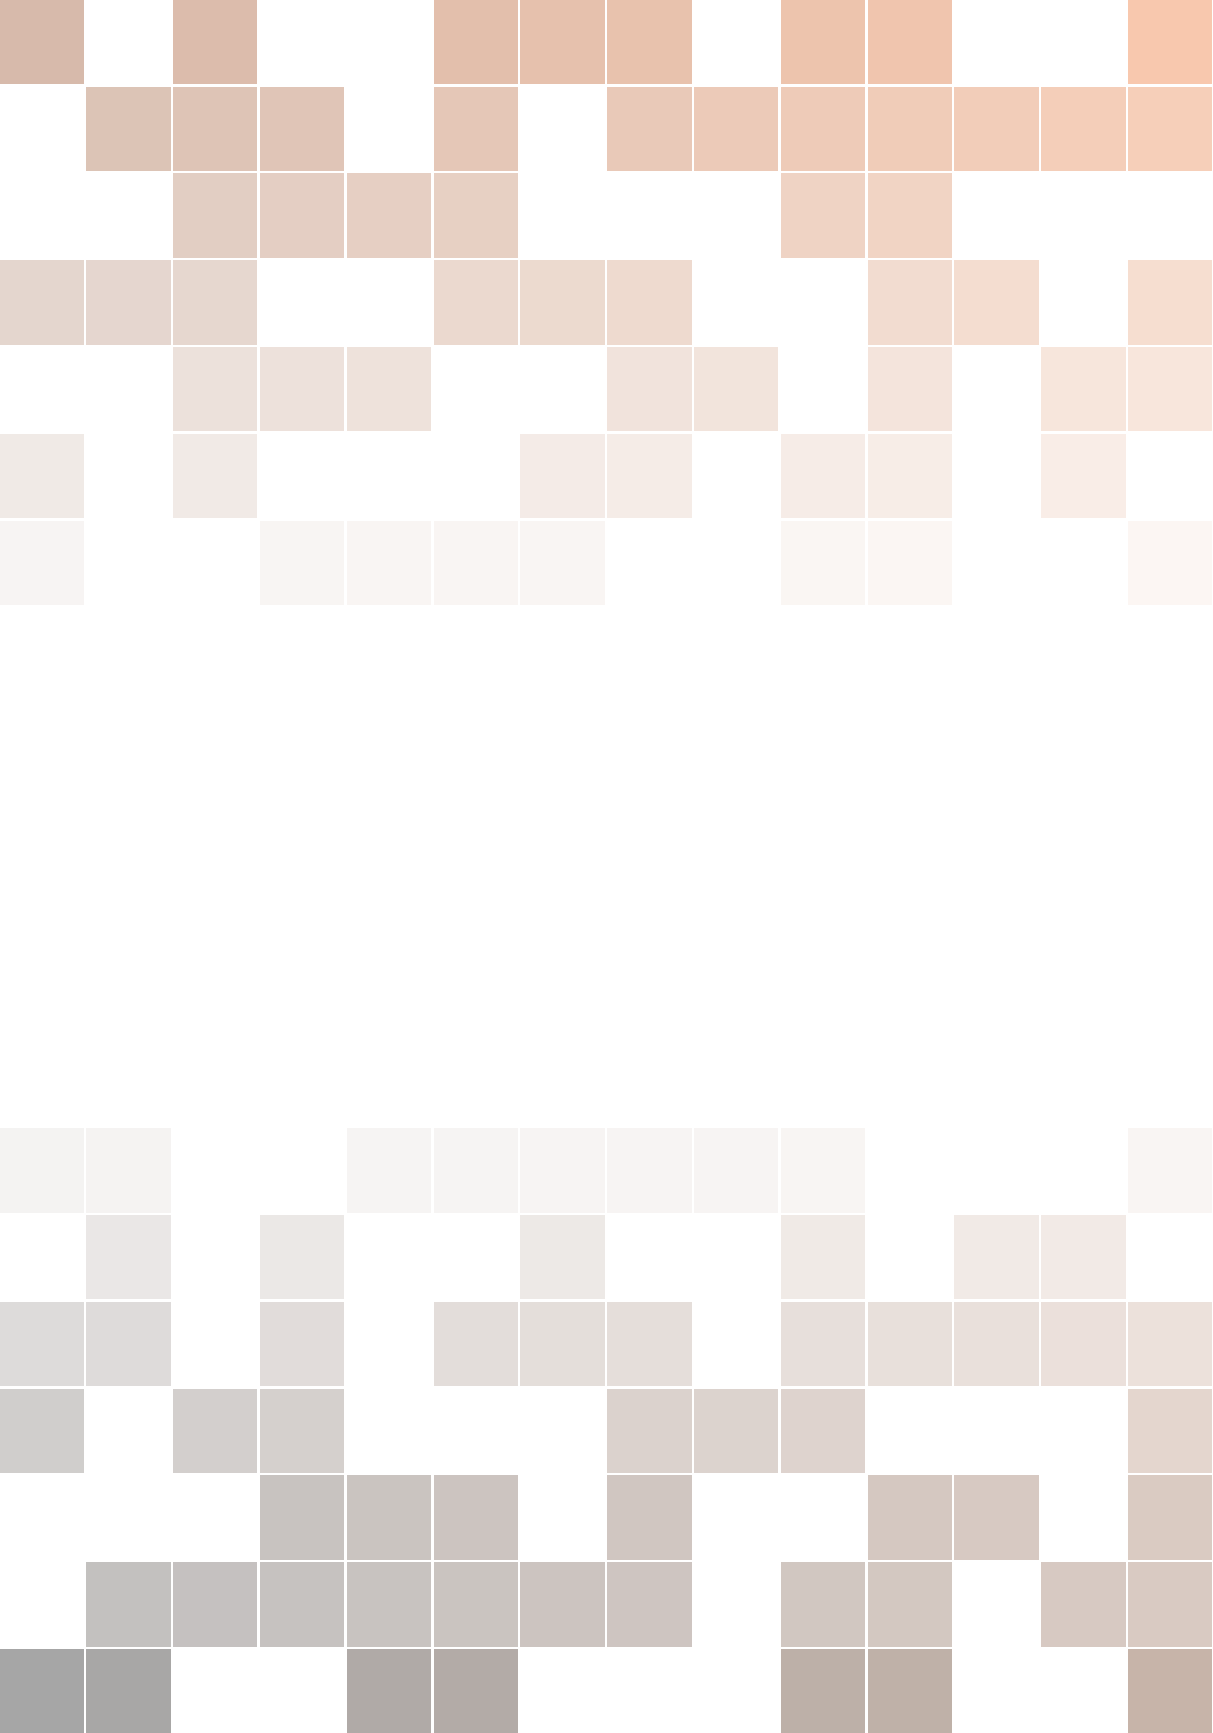
\includegraphics[width=\paperwidth]{poly/Pictures/background.pdf}};
\draw (current page.center) node [fill=ocre!30!white,fill opacity=0.6,text opacity=1,inner sep=1cm]{\Huge\centering\bfseries\sffamily\parbox[c][][t]{\paperwidth}{\centering Signal et Filtrage\\[15pt] % Book title
{\Large IMACS 2ème année}\\[20pt] % Subtitle
{\huge Alexandre Boyer \& Pascal Acco }}}; % Author name
\end{tikzpicture}
\vfill
\endgroup



% -------------------------------------------------------------------------
%	TABLE OF CONTENTS
%-------------------------------------------------------------------------
\usechapterimagefalse 
%\pagestyle{empty} % Disable headers and footers for the following pages
%\tableofcontents % Print the table of contents itself
%\cleardoublepage % Forces the first chapter to start on an odd page so it's on the right side of the book
\pagestyle{fancy} % Enable headers and footers again

%-------------------------------------------------------------------------
%	CHAPITRES
% -------------------------------------------------------------------------

\tableofcontents
\setcounter{tocdepth}{4}
\cleardoublepage

\chapter{Les bases de Fourier}
\label{chap:fourier}
Ce chapitre présente les transformées, séries de \Fourier{} et introduit la transformée de\Fourier{} Discrète en se basant sur une vision d'espace vectoriel Euclidien.

\section{Espaces vectoriels normés pour les fonctions}
Les produits scalaires pour différents espaces de fonctions sont définis et illustrés dans la \tabref{tab:scalaires}
\begin{table}[htbp]
  % \arraystretch=1.2
  \centering
  \begin{tabular}{p{0.1\textwidth}|c|c}
                      &Support infini    & Support fini ou périodique  \\\hline
                      &  \begin{tabular}{c} \graphe{0.4\textwidth}{fonction_rc}\end{tabular}
   &  \begin{tabular}{c} \graphe{0.5\textwidth}{fonction_rtc} \end{tabular}                           \\
    variable continue & $f:\R\mapsto\C$    &  $f:\RT0{}\mapsto\C\;$  ou $f:\;[0,\,T_0[\, \mapsto \C $       \\
    &$\scal{f}{g}=\intDt{\R}{}{f(t).\conj{g(t)}}$ $\quad\deDim{\frac{V^2}{\Hz}}$ & $\scalp{f}{g}=\frac{1}{T_0}\intDt{0}{T_0}{f(t).\conj{g(t)}}$ $\quad\deDim{V^2}$ \\\hline
                      &   \begin{tabular}{c} \graphe{0.4\textwidth}{fonction_nc}\end{tabular}
   &  \begin{tabular}{c} \graphe{0.5\textwidth}{fonction_znc}    \end{tabular}                        \\
    variable discrète & $\N\mapsto\C$    &  $\ZN0\mapsto\C\;$  ou $\;\semiN{0}{N}\;\mapsto \C$        \\
                      & $\scald{f}{g}=\somme{k\in\N}{}{f[k].\conj{g[k]}}$ $\quad\deDim{V^2}$& $\scaldp{f}{g}=\somme{k=0}{N-1}{f[k].\conj{g[k]}}$  $\quad\deDim{V^2}$  
  \end{tabular}
  \caption{Les produits scalaires adaptés aux différents espaces de fonctions. Par clarté, on ne représente que le module de la fonction qui est dans la cas général complexe.}
  \label{tab:scalaires}
\end{table}

\begin{remarque}\remarqueTitre{Pour quoi du complexe pour du réel ?}
  On considère le cas général des fonctions à valeurs dans $\C$ car cela permet~:
  \begin{itemize}
  \item de représenter des signaux de type phaseur (vecteurs en rotation)
  \item de représenter facilement des signaux réels dont la bande de
    fréquence est finie (signaux dits \emph{bande étroite})
  \item de pouvoir appliquer la trasnformée de \Fourier{} à une
    transformée de \Fourier{} (qui est complexe même pour des signaux
    réels) et de voir l'opération de transformée comme un isomorphisme
    et de jouer avec la notion de dual.
    \end{itemize}
  \end{remarque}
  
  
  \begin{exercice}\exerciceTitre{Propriété de scalaire et norme dans le cas général}
  On aurait pu définir ces produits scalaires en ne prenant jamais le
  conjugué d'une fonction $g$ (ou en considérant des fonction à valeurs réelles de manière à ignorer ce conjugué car $\conj{g}=g$).
  \begin{enumerate}
  \item Vérifiez dans le cas réel (sans conjugué) que le produit $\scal{f}{g}$ à les propriété d'un produit scalaire, en déduire la norme induite $\|f\|^2=\scal{f}{f}$ et déterminer la dimention de $\|f\|^2$ : est-ce de la puissance ou de l'énergie, est-ce une valeur ou une densité ?
  \item Appliquez cette norme (toujours sans le conjugué) au signal imaginaire pur
    $f: t\mapsto i$. Quelle propriétée de la norme n'est pas respectée ?
  \item Refaites de même en prenant cette fois-ci les formules de
    \tabref{tab:scalaires} avec le conjugué de $g$ et vérifiez que
    cette propriété est vérifiée dans le cas général des fonctions à
    variables complexes.
  \item Vérifiez que $\scal{f}{g}=\conj{\scal{g}{f}}$ et que donc le produit scalaire est linéaire à gauche $\forall\lambda\in\C,\; \scal{\lambda\,f}{g}=\lambda\scal{f}{g}$ et \emph{à moitié linéaire} à droite $\forall \lambda\in\C,\; \scal{f}{\lambda\,g}=\conj{\lambda}\scal{f}{g}$
  \end{enumerate}
On comprend maintenant pourquoi, dans le cas général des fonctions à valeurs complexes, on utilise le conjugué dans l'expression des produit scalaires et pourquoi on parle de produit \emph{sesqui--linéaire} pour ces produits scalaires~: \emph{sesqui} en latin voulant dire \og{}un et demi\fg{} en latin.  
\end{exercice}

\subsection{Analyse et synthèse de fonctions dans une base}

Par anlogie avec les espaces vectoriels Euclidiens, on va pouvoir manipuler les fonctions comme indiqué dans la \tabref{tab:hilbert}.


%\begin{landscape}
\begin{table}[htbp]
\renewcommand{\arraystretch}{1.4}
\begin{tabular}{p{0.1\textwidth}|p{0.32\textwidth}|p{0.6\textwidth}}
  & Euclidien fini & Espace de fonctions \\\hline
  Base   Ortho--normée & une base finie de vecteurs $$\B=\p{\vec{e_n}}_{n\in\ZN0}$$ normés $\|\vec{e_n}\|=1$ et orthogonaux $\scal{\vec{e_n}}{\vec{e_m}}=0$ & base dénombrable de fonctions $\p{\vec{w_n}}_{n\in\N}$ ou indénombrable $\p{\vec{w_f}}_{f\in\R}$ repérées par leur fréquences $f$ ou un indice $n$ associé~;  fonctions d'énergie unitaire $\|\vec{w_n}\|=1$ ou $\|\vec{w_f}\|=1$, et orthogonales $\scalp{\vec{w_n}}{\vec{w_m}}=0$ ou $\scal{\vec{w_{f}}}{\vec{w_{f'}}}=0$\\\hline
  
  Analyse &  décomposer un vecteursdans cette base en coefficients $V_n=\scal{\vec{v}}{\vec{e_n}}$ et en donner les coordonnées $$\caCest{\vecDs{V}{\B}}{\rightleftharpoons\vec{v}}=\vvvectBase{V_0=\scal{\vec{v}}{\vec{e_0}}}
            {\vdots}
            {V_{N-1}=\scal{\vec{v}}{\vec{e_{N-1}}}}{\B}$$
                   &  décomposer une fonction $\vec{u}$ en fréquentiel avec la transformée $U(f)$ ou avec les coéfficients $U(n)$ de la série~: $$U(f)=\scal{\vec{u}}{\vec{w_f}}=\scalint{u(t)}{w_f(t)}{t}$$ $$U(n)=\scalp{\vec{u}}{\vec{w_n}}=\scalpint{u(t)}{w_n(t)}{t}$$ \\\hline
  
  Synthèse &  recomposer un vecteur dans cette base $\vec{v}=\somme{k\in\ZN0}{}{\caCest{U_0}{\scal{\vec{v}}{\vec{e_0}}}}\,.\,\vec{e_0}$ \graphe{4cm}{projections} &  recomposer une fonction par transformation inverse de $U(f)$  ou recompostion de série $U(n)$~: $$\vec{u}(t) = \int\limits_{-\infty}^{\infty}{\caCest{U(f)}{\scal{\vec{u}}{\vec{w_f}}}\,.\,\vec{w_f}(t)\,\dt} $$ $$\vec{u}(t)=\sum\limits_{n\in\N}\caCest{U(n)}{\scalp{\vec{u}}{\vec{w_n}}}\,.\,\vec{w_n}(t) $$\\\hline

  Projeter avec Plancherel  &  calculer le produit scalaire de vecteurs par leurs composantes~: $$\scal{\vec{u}}{\vec{v}}=\scal{U_{\B}}{V_{\B}}=\Tr{\vecDs{U}{\B}}\,.\,\vecDs{V}{\B}$$ $$\caCest{\hhhect{U_0}{\ldots}{U_{N-1}}}{\Tr{\vecDs{U}{\B}}}\,.\,\vvvect{V_0}{\vdots}{V_{N-1}}$$
  % au lieu de calculer $$\scal{\vec{u}}{\vec{v}}=\|\vec{u}\|\,\|\vec{v}\|\,\cos\p{\alpha}$$
                   &  on peut calculer un produit scalaire (utile aux correlations et convolutions) à partir de sa transformée ou composantes de la série~: $$\scal{\vec{u}}{\vec{v}}=\scalint{u(t)}{v(t)}{t} = \scal{U}{V} =  \scalint{U(f)}{V(f)}{f}$$ $$\scalp{\vec{u}}{\vec{v}}=\scalpint{u(t)}{v(t)}{t} = \scaldp{U}{V} =  \scalpdint{U(k)}{V(k)}{k}$$
  \\\hline
  
  Normer avec Parseval  &  Calculer la norme en sommant les carrés des coordonnées~: $$\|\vec{u}\|^2=\|U_{\B}\|^2=\sum {U_n}^2$$ &  calculer la puissance moyenne par la transformée $u(f)$ ou en sommant celle des composantes fréquentielles $U(n)$~: $$\|\vec{u}\|^2=\|U\|^2=\int\limits_{-\infty}^{\infty}{|u(t)|^2\dt}=\int\limits_{-\infty}^{\infty}{|U(f)|^2\df} $$  $$\|\vec{u}\|^2=\|U\|_P^2=\frac{1}{T_0}\int\limits_{0}^{T_0}{|u(t)|^2\dt}=\sum\limits_{k\in\N}{|U(k)|^2} $$
\end{tabular}

\caption{Structure Euclidiene à structure de Hilbert}
\label{tab:hilbert}
\end{table}
%\end{landscape}

\subsection{Base de la \TF{}}

La \TF{} (Transformée de \Fourier), ou \FT{} (\emph{Fourier
  Transform}) en anglais, s'applique aux fonction continues et utilise
une base d'ondes complexes
$\Bf=\p{\caCest{t\mapsto e^{i 2 \pi\,f\,t}}{w_f}}_{f\in\R}$.

\begin{exercice}
Tentez de retrouver la formule de la transformée et son inverse et d'esquisser le schéma ci-dessous sans le regarder, en se rappelant juste que c'est une application de $$\R\rightarrow\C\;\;\operateur{\TF}\;\;\R\rightarrow\C$$ basée sur le produit scalaire continu noté $\scal{}{}$ avec la base continue $\Bf=\p{w_f}_{f\in\R}$
\end{exercice}

\graphe{\textwidth}{tf}

 On peut faire
l'analogie avec les espaces Euclidiens mais pas l'amalgame, car~:
\begin{itemize}
\item le produit scalaire $\scal{}{}$ est défini  dans le cas de fonctions de carré
intégrable, ou \emph{fonction à énergie finie}, que nous notons $\Leb{2}$,
\item les vecteurs de la base ne sont pas normés car de norme infinie~;
\item la base n'est pas finie, ni infinie dénombrable mais infinie indénombrable.
\end{itemize}

Mais lorsque l'on se place dans le cas de fonctions de carré
intégrable, ou fonction à énergie finie, que nous notons $\Leb{2}$,
l'espace est complet (les suites de Cauchy convergent) dont les sommes
infinies se comporte bien dans $\Leb{2}$~: c'est une espace de
Banach. De plus le produit scalaire associé à la norme 2 existe et on
a donc un espace de \Hilbert{} où la norme et le produit scalaire sont
des application linéaire dans $\Leb{2}$. Comme il s'agit d'une espace
de dimention infinie, il ne suffit pas d'avoir une base de dimention
infinie pour couvrir tout l'espace, mais dans le cas de $\Leb{2}$ avec
la base $\Bf$ on montre que tout l'espace est engendré.

Bref ! ça fonctionne tout comme un espace Euclidien sans en être un.

\begin{exercice}
Prendre la base $\Bf=\p{w_f}_{f\in\R}$ et utiliser la partie espace indénombrable de la \tabref{tab:hilbert} pour retrouver les formules de \Plancherel{} et \Parseval{}. 
\end{exercice}


\subsection{Base des \sdf{}}
Les \sdf{} (Séries de \Fourier{}), ou \FS{} (\emph{Fourier Series}) s'appliquent aux fonctions continues périodiques et   utilisent une base d'ondes complexes dénombrable $\Bf=\p{\caCest{t\mapsto e^{i \frac{2 \pi}{T_0}\,n\,t}}{w_{T_0}^n}}_{n\in\N}$.
\begin{exercice}
Tentez de retrouver la formule de la décomposition et recomposition en \sdf{} et d'esquisser le schéma ci-dessous sans le regarder, en se rappelant juste que c'est une application de $$\RT0\rightarrow\C\;\;\operateur{\sdf}\;\;\N\rightarrow\C$$  basée sur le produit scalaire continu périodique noté $\scalp{}{}$ et avec la base discrète $\Bf=\p{W_{T_0}^n}$.
\end{exercice}

\graphe{\textwidth}{sdf}

 On peut faire l'analogie avec les espaces Euclidiens mais pas l'amalgame, car~:
 \begin{itemize}
   \item le produit scalaire $\scalp{}{}$ est défini dans le cas de fonctions périodiques de carré intégrable, \emph{fonctions de puissance moyenne finie},  que nous notons $\LebP{2}$
 \item ce n'est pas un isomorphisme car on passe d'un espace continu périodique à
   un espace discret~! La transformée inverse se fait avec le produit scalaire discret $\scald{}{}$
\item la base n'est pas finie, mais infinie dénombrable~;
\end{itemize}

Bref ! cela fonctionne un peu comme un espace Euclidien fini sans en être un...

\begin{exercice}
  Prendre la base  $\Bf=\p{t\mapsto \cos\p{\frac{2 \pi}{T_0}\,n\,t}}_{n\in\Z}\cup \p{t\mapsto \sin\p{\frac{2 \pi}{T_0}\,n\,t}}_{n\in\Z^*}$, et voir que l'on retrouve les formules \textbf{à un facteur 2 près !} Et oui ! La base n'est pas normée car un rapide calcul montre que la norme des vecteurs vaut $2$.

  En prenant $\Bf=\p{t\mapsto\frac{\cos\p{\frac{2 \pi}{T_0}\,n\,t}}{\sqrt{2}}}_{n\in\Z^*}\cup \p{t\mapsto \frac{sin\p{\frac{2 \pi}{T_0}\,n\,t}}{\sqrt{2}}}_{n\in\Z^*} \cup \p{t\mapsto 1}$ on obtient une définition des \sdf{} chère aux physiciens. On peut ne pas normer les vecteurs mais prendre des pincettes et modifier les formules...
\end{exercice}

\subsection{Base de la \TFSD{}}

La \TFSD{} (Transformée de \Fourier{} des Signaux Discrets), ou \DTFT{} (\emph{Discrete Time Fourrier Transform} en anglais, s'applique aux fonctions à variable discrète et utilise une base d'ondes complexes indénombrable $\Bf=\p{\caCest{k\mapsto e^{i 2 \pi\,f\,k\,T_e}}{w_{T_e}^f}}_{f\in\SFe{}}$.

\begin{exercice}
Tentez de trouver la formule de cette \TFSD{}  et son inverse, d'esquisser le schéma ci-dessous sans le regarder, en pensant que c'est la \og{}duale\fg{} de la \sdf{}. Il s'agit d'une application de $$\N\rightarrow\C\;\;\operateur{\TFSD}\;\;\RFe\rightarrow\C$$ basée sur le produit scalaire discret noté $\scald{}{}$ avec la base continue $\Bf=\p{w_f}_{f\in\SFe}$
\end{exercice}

\graphe{\textwidth}{tfsd}


On peut difficilement faire l'analogie avec les espaces Euclidiens  car~:
\begin{itemize}
   \item le produit scalaire $\scald{}{}$ fonctionne dans le cas de suites discretes absoluement convergentes~;
 \item ce n'est pas un isomorphisme car on passe d'un espace discret à un espace continu périodique~! La transformée inverse se fait avec le produit scalaire continu périodique $\scalp{}{}$ (Attention la période dans l'espace des fréquences est $F_e$)~;
\item la base n'est pas finie, ni dénombrable  mais infinie indénombrable.
\end{itemize}


\begin{exercice}
  On admet pour le moment que la \TFSD{} d'un signal $s[k]$ quelconque est une fonction $S(f)$ de période $F_e$. On peut donc voir $S(f)$ comme une fonction de période $F_e$ de la variable réelle $f$ et y appliquer une décomposition en séries de \Fourier{}!

  Faites-le et comparez avec la \TFSD{} inverse. Vous venez de basculer dans un dual ! D'ailleurs on peut voir $s[k]$ comme les coefficients de \Fourier{} d'une fonction de fréquence fondamentale $T_E$ et appliquer une recomposition de la série et trouver $S(f)$.

  Donc \TFSD{}=\sdf{}$^{-1}$ et inversement \sdf{}=\TFSD{}$^{-1}$
\end{exercice}

\subsection{Base de la \TFD{} et  \FFT{}}

La \TFD{} (Transformée de \Fourier{} Discrète), ou \DFT{} (\emph{Direct Fourier Transform}) en anglais, s'applique aux fonctions discrètes à support fini et utilisent une base d'ondes complexes discrète finie $\Bf=\p{\caCest{k\mapsto e^{i \frac{2 \pi}{N}\,n\,k}}{W_N^{nk}}}_{n\in\SN0}$.

La $\FFT{}$ (\emph{Fast Fourier Transform} en anglais uniquement) est un algorithme efficace de calcul de la \TFD{}~: c'est donc la même transformation avec les mêmes valeurs~!

\begin{exercice}
Tentez de trouver la formule de cette \TFD{}  et son inverse, d'esquisser le schéma ci-dessous sans le regarder. Il s'agit d'une application de $$\SN0\rightarrow\C\;\;\operateur{\TFD}\;\;\SN0\rightarrow\C$$ basée sur le p.s. discret périodique noté $\scaldp{}{}$ avec la base continue $\Bf=\p{w_Nnk}_{n\in\SN0}$
\end{exercice}

\graphe{\textwidth}{tfd}



On peut faire l'analogie avec les espaces Euclidiens finis et \textbf{on peut faire l'amalgame~!} car c'en est un mais dans $\C$ donc~:
\begin{itemize}
\item le produit scalaire n'est pas symétrique mais \og{}symétrique et demi\fg{} \cad \emph{sesquilinéaire} car $\scal{u}{v}=\conj{\scal{v}{u}}$.
\end{itemize}

\begin{remarque}\remarqueTitre{Base pas normée}
  Le terme $W_N= e^{-i \frac{2 \pi}{N}}$ est en fait une racine $N$ième de l'unité. Le calcul de la norme du vecteur $n$ de la base $\|w_n=k\mapsto W_N^{-nk}\|^2$ devient donc $$\scaldp{w_n}{w_n}=\somme{k=0}{N-1}{e^{i \frac{2 \pi}{N}nk}\,.\,e^{-i \frac{2 \pi}{N}nk}} =\somme{k=0}{N-1}{1}=N $$

  Une formulation normée et symétrique de la \TFD{} ferait donc intervenir un facteur $\frac{1}{\sqrt{N}}$ pour la \TFD{} et son inverse. Pour des raisons de simplicité et de contrainte de calcul numérique, la formulation non normée de la figure est largement utilisé. La \TFD{} n'est pas divisée par $\sqrt{N}$ et donc apparait le terme $\frac{1}{N}$ dans la \TFD{} inverse.
\end{remarque}

\begin{exercice}
  Tout comme la \TF{}, la \TFD{} est un isomorphisme bidual. Pour un
  signal $s$ quelconque, calculez la transformée de la transformée et
  montrez que
  $ \caCest{\F\circ \F}{\F^2}\b{s}=\F\b{\F\b{t\mapsto s(t)}} =
  t\mapsto s(-t)$. Donc si on recalcule deux fois la transformée on obtient le signal d'origine et on montre que $\F^2$ est sa propre réciproque. Déduisez une technique pour calculer la transformée inverse $\F^{-1}$ en utilisant la transformée $\F$.

  Faites de même pour la \TFD{} 
\end{exercice}




%%% Local Variables:
%%% mode: latex
%%% TeX-master: "main"
%%% End:

\chapter{Systèmes discrets}


L'analogie avec les systèmes continus est forte, nous étudions de-même
le cas des systèmes discrets linéaires invariants dans le temps avec
une vision par opérateurs.


\section{Systèmes linéaires}

\begin{definition}{Système SISO (Single Input Single Output)}
  
  Un système discret SISO (resp. continu SISO) relie à un signal d'entrée $x$
  un signal de sortie unique $y$. Les signaux $x$ et $y$ sont des
  fonctions de la variables réelle discrète $k$ (resp. $t$) appartenant
  à un espace de fonction le plus général possible noté ici $L_E$.

  La relation entrée-sortie est donc modélisée par une application
  mathématique de $L_E$ dans $L_E$ notée $L$ (resp. $L_c$ en continu)
  et définie ainsi~:
  \begin{eqnarray}
    L : \qquad \application{L_E}{L_E}{x : \; k\mapsto x\b{k}\quad{}}{\quad y :\; k\mapsto y\b{k}} \\
    L_c: \qquad \application{L_E}{L_E}{x : \; t\mapsto x\p{t}\quad{}}{\quad y :\; t\mapsto y\p{t}} 
    % DONE : correction TYPAGE et remarque notation
  \end{eqnarray}
\end{definition}

Une classe de système fondamentale est la classe des systèmes
linéaires car elle offre de nombreux outils et propriétés
mathématiques.

\begin{definition}{Système linéaire}
  \label{def:linearite}
  
  Une système est dit linéaire si, et seulement si, l'application $L$
  associée est linéaire, soit pour tout
  $\p{x_1,x_2,\lambda} \in L_E^2 \times \R$~:
  \begin{eqnarray}
    \label{eq:def_linearite}
    \forall t \in \R \qquad L\b{x_1 + \lambda\, x_2}(t) = L\b{x_1}(t) + \lambda\,L\b{y_2}(t) \nonumber\\
    \iff \qquad L\b{x_1 + \lambda\,x_2} = L\b{x_1} +\lambda L\b{x_2 }
  \end{eqnarray}
\end{definition}

Une des conséquences de la linéarité est la possibilité d'appliquer le
principe de superposition cher à l'électronicienne~: \og{} la réponse
du système à une combinaison linéaire d'entrées est la combinaison des
réponses de chaque entrée.\fg{}

\begin{definition}{Systèmes continus élémentaires}
  \label{def:systeme_elementaires_continus}
  
Les trois systèmes linéaires élémentaires que nous considérons dans
l'étude des systèmes linéaires continus sont :
\begin{description}
\item[le gain $a.x$]~: $t \mapsto a\,x\p{t}$ où a est une constante
  scalaire réelle ou complexe
\item[le dérivateur $\oder\b{x}=\oder\circ x$]~: $ t \mapsto \dDtDe{x}\p{t} $
\item[l'intégrateur $\oint\b{x}=\oint\circ x$]~: $ t \mapsto \integ{0}{t}{x\p{\nu}\derivDe{\nu}}$ 
\end{description}
\end{definition}

On peut aisément vérifier que ces systèmes respectent la condition de
linéarité~\ref{eq:def_linearite}.

\begin{remarque}
  De manière implicite, on choisi un espace de fonction $L_c$ qui est
  stable par toute combinaison de compositions de ces opérateurs (même
  une infinité de composition de $\oder$ par exemple) soit un espace
  complet de fonctions.

  On aimerait que les opérateurs dérivateur $\oder$ et intégrale
  $\oint$ commutent et soient réciproque sur $L_c$~:
  $\oder\circ\oint=\oint\circ\oder=\Id$. De manière à obtenir une
  composition de ces opérateurs qui ait la même propriété qu'un
  produit algébrique inversible.
  
  Pour que cela soit vrai même avec les fonctions discontinues, il
  faut introduire les distributions de \Dirac{} voir
  \chapref{sec:deriv_discontinues}.
\end{remarque}

\begin{definition}{Systèmes élémentaires discrets}
  
Dans le cas des systèmes discret, les systèmes élémentaires sont :
\begin{description}
\item[le gain $a.x$]~: $ k \mapsto a\,x\b{k}$ où a est une constante
  scalaire réelle ou complexe
\item[le retard unité $\oret\b{x}=\oret\circ x$]~: $ k \mapsto x\b{k-1}$.
\item[l'avance unité $\oavance\b{x}=\oavance\circ x$]~: $ k \mapsto x\b{k+1} $ 
\end{description}
\end{definition}

On peut aisément vérifier que ces systèmes respectent la condition de
linéarité~\ref{eq:def_linearite}.

\begin{remarque}
  La commutation et réciprocité des opérateurs retard $\oret$ et
  avance $\oavance$ est évidente et ne pose pas de problème théorique,
  contrairement au cas continus~:
  $\oret\circ\oavance=\oavance\circ\oret=\Id$.

  La composition~$\circ$ de ces opérateurs avec l'opérateur somme de
  systèmes $+$ a donc une structure d'anneau commutatif~: $\circ$ et
  $+$ des systèmes se comporte comme $\times$ et $+$ des nombres
  réels.

  L'espace des signaux $L_e$ (ou des suites complexes) est stable et
  complet par l'application des opérateurs élémentaires.
\end{remarque}

L'opérateur dérivée n'as pas de sens en discret car la limite
$s'(x)=\lim\limits_{h\to 0} \frac{s(x+h)-s(x)}{h}$ n'aurait pas de
sens pour $h$ entier. On peut s'approcher de cet opérateur avec des
combinasons plus ou moins complexes et précises des opérateusr avance et
retard élémentaires.

\begin{exemple}
  \label{exemple:differentiateur_lineaire}
  L'effet du système \emph{différentiateur} sur le signal d'entrée est d'écrit par
  l'opérateur ~: $$L : x \mapsto y=\frac{x-\oret\b{x}}{T_e}$$
  
  Vérifions d'abord que cet opérateur est linéaire~:
  \begin{eqnarray*}
    L\b{x_1+\lambda x_2}\b{k} &= L\b{x_1+\lambda x_2}\b{k}\\
                              &= \frac{x_1\b{k}+\lambda x_2\b{k} - \oret\b{x_1+\lambda x_2}\b{k}}{T_e}\\
                              &= \frac{x_1\b{k}+\lambda x_2\b{k} - \p{x_1\b{k-1}+\lambda x_2\b{k-1}}}{T_e} = A\\
    L\b{x_{1}}\b{k}+\lambda\,L\b{x_{2}}\b{k}  &= \frac{x_1\b{k} - x_1\b{k-1}}{T_e}+\lambda\,\frac{x_2\b{k} - x_2\b{k-1}}{T_e}=A
  \end{eqnarray*}
  Le système est donc linéaire.
\end{exemple}


% \begin{remarque}
%   Pour résoudre les complexes équations différentielles des
%   télégraphistes, \Heaviside{} utilise ces opérateurs de base et
%   introduit le \emph{calcul opérationnel}. Cela consiste à représenter
%   l'application de l'opérateur dérivée sur une fonction $f$ comme une
%   simple multiplication par un nombre $p$. Ainsi une équation
%   différentielle $a\,y'' + 2y' -y = 3\int x$ est associée à l'équation
%   symbolique $a\,p^2\,y + 2\,p\,y - y = \frac{3}{p}x$. Il est alors
%   possible de résoudre algébriquement l'équation sous forme de
%   fractions rationnelles ce qui donnerait avec notre exemple~:
%   $y = \frac{3/p}{a\,p^2+2p+1} x$. Rappelons que $x$ et $y$ sont des
%   fonctions et non des réels et que dans ce cas les opérations ne sont
%   pas de simple multiplication et addition de réels mais bien des
%   multiplications et additions de fonctions. La variable symbolique
%   $p$ est utilisée comme un nombre réel mais n'est en aucun cas un
%   réel...
% \end{remarque}

\section{Systèmes invariants}
Il est fréquent, et surtout théoriquement utile, qu'un système
réagisse de la même manière indépendemment de l'instant où est
appliqué le signal d'entrée. Ce qui conduit à la définition suivante~:
\begin{definition}{Système invariant dans le temps}
  Un système discrète (resp. continu) est dit invariant dans le temps si et seulement
  si son application associée $L$ (resp. $L_c$) vérifie~:
  \begin{eqnarray}
    \forall x\in L_E, \forall (k,k_0)\in \N^2, \quads L[k\mapsto x(k-k_{0})] = L[x](k-k_{0}) \\
    \forall x\in L_E, \forall (t,t_0)\in \R^2, \quads L_c[t\mapsto x(t-t_{0})] = L[x](t-t_{0}) 
  \end{eqnarray}
  
  En terme d'opérateur~;  un système $L$ est invariant dans
  le temps si, et seulement si, son opérateur commute avec  tout opérateur
  retard de $k_0$ noté $\oretDe{k_0}=\oret^{k_0}\b{x}= k\mapsto x\b{k-k_0}$~:
  \begin{eqnarray}
    \label{eq:sys_invariant}
    L\circ\oretDe{k_0} \; = \; \oretDe{k_0}\circ L  \qquad \iff \qquad  L\b{\oretDe{k_0}\b{x}} = \oretDe{k_0}\b{L\b{x}}
    \\
    L_c\circ\oretDe{\tau} \; = \; \oretDe{\tau}\circ L_c  \qquad \iff \qquad  L_c\b{\oretDe{\tau}\b{x}} = \oretDe{\tau}\b{L_c\b{x}}
  \end{eqnarray}
\end{definition}

Autrement dit \og{}la réponse du système à un signal retardé est le
retard de la réponse du système.\fg{}~; ou encore \og{} la réponse du
système ne dépend pas de l'origine des temps choisie.\fg{}


%% TODO lien vers causalité.

\begin{remarque}
  Il est facile de vérifier que les systèmes discrets élémentaires que
  sont le gain~; le retard unitaire et l'avance unitaire (gain,
  dérivateur et intégrateur pour le continu) sont invariants.  Il en
  est de même pour tout système constitué de combinaisons linéaires
  et de composition de systèmes élémentaires.
  
  Il suffit alors de montrer que le système se décompose avec des
  \emph{coefficients constants} avec des systèmes élémentaires en le
  mettant sous forme \emph{d'équation aux différences} ou
  \emph{récurrence} à coefficients constants (\emph{equations
    différentielle} en continu) ou en un schéma bloc à coefficients
  constant.
\end{remarque}


\section{Réponse d'un système LTI}
Rappelons qu'un système peut aussi bien représenter un correcteur dans
une boucle d'asservissement, qu'un filtre utilisé en boucle ouverte,
ou bien un modèle de système à commander ou observer~: calculer la
réponse d'un système à un signal c'est aussi  \og{}faire du
filtrage.\fg{}

Nous allons d'abord montrer que l'opération de filtrage consiste en
temporel à effectuer une convolution du signal d'entrée $x$ avec la
réponse impulsionnelle $h$ du système $H$ ainsi défini.

En un second temps nous utiliserons la réponse impulsionnelle pour
caractériser la propriété de stabilité du système.

Nous terminerons en montrant que l'opération duale du filtrage
temporel est un \emph{fenêtrage fréquentiel} ou multiplication par la
transformée de la réponse impulsionnelle $\TZ\p{h}=\TZlui{H}$.

\subsection{Réponse impulsionnelle}
Dans le cas discret, l'obtention de la réponse d'un système est facile
à obtenir en utilisant les propriétés LTI du système $H$ et en
décomposant le signal d'entrée $x$ dans la base temporelle canonique.


Contrairement au cas continu, un signal d'entrée quelconque $x$ se
décompose facilement en impulsions unité. La
\figref{fig:reponse_convolution} reprend la décomposition en
impulsions d'un signal d'entrée nommé $s$
\eqref{eq:decomposition_unite} et applique un système $H$ de réponse
impulsionnelle $h$ à chaque impulsion pour obtenir la réponse $y$ du
système. On retrouve ainsi la formule de convolution temporelle de
$y=s\conv h$. Le résultat est démontré dans l'équation
\eqref{eq:reponse_convolution} en utilisant les propriétés de
linéarité et invariance du système.

\begin{figure}[ht!]
  \centering \graphe{0.9\textwidth}{reponse_convolution}
  \caption{La réponse d'un système linéaire invariant $y$ est la somme
    des réponses impulsionnelles des impulsions qui composent le
    signal d'entrée $s$.}
  \label{fig:reponse_convolution}
\end{figure}

\begin{align}
  \label{eq:reponse_convolution}
  \caCest{x = \somme{j=-\infty}{\infty}{x\b{j}\delta_{j}}}{\text{signal}}\quad \implies\quad &y=H\b{x}=H\b{\somme{j=-\infty}{\infty}{x\b{j}\delta_{j}}} \nonumber\\
  \underset{\text{linéarité de H}}{\implies}\quad &y=\somme{j=-\infty}{\infty}{H\b{ \;\caCest{x\!\!\b{j}}{\text{constante !}}\delta_{j}\;}} \underset{\text{linéarite de H}}{=} \;\;\somme{j=-\infty}{\infty}{x\!\b{j}\caCest{H\b{\delta_j}}{H.\oret^j\b{\delta_0}}} \nonumber \\
  \implies \quad &y=\somme{j=-\infty}{\infty}{x\b{j}.H.\oret^j\!\b{\delta_{0}}} \underset{\text{invariance de H}}{=} \;\;\somme{j=-\infty}{\infty}{x\b{j}.\oret^j\,.\,\caCest{H\b{\delta_{0}}}{h}}\nonumber\\
  \implies \quad & y= \somme{j=-\infty}{\infty}{x\b{j}.\caCest{\oret^j\b{h}}{k\mapsto h\b{k-j}}}=x\conv h \nonumber\\
  \implies \quad & \forall k\in\Z,\quad  y\b{k}= \somme{j=-\infty}{\infty}{x\b{j}\,h\!\b{k-j}} = x\conv h\b{k}
\end{align}
où l'opérateur $\conv$ est la convolution discrète définie ci-après.

\begin{definition}{Convolution discrète}
  \label{def:convolution_discrete}
  
  La convolution de signaux discret $u$ et $v$ notée $u\conv v$ est le
  signal discret défini par~:
  \begin{align}
    \label{eq:convolution_discrete}
    &u\conv v \quad &:& \quad k \mapsto u\conv v\b{k} =\somme{j=-\infty}{\infty}{u\ded{j}.v\ded{k-j}} &\underset{j\leftrightarrow j+k}{=}&  \somme{j=-\infty}{\infty}{u\ded{j+k}.v\ded{-j}} \nonumber\\
    &u\conv v \quad & = &\quad\scald{u}{\caCest{\conj{\oret^k.\,\Sy\ded{v}}}{\conj{j\mapsto v\ded{k-j}}}} &=& \scald{\oret^{-k}\ded{u}}{\conj{\Sy\ded{v}}} 
  \end{align}
  où $\oret^k$ est le retard de $k$ échantillons et
  $\oret^{-k}=\oavance^k$ son opérateur réciproque (inverse
  algébrique)~: l'avance de $k$ échantillons.
\end{definition}

\begin{remarque}
  \textbf{Attention à l'ordre des opérations~: la symétrie et le
    retard ne commutent pas~!}

  Même si nous avons vu dans \secref{sec:dualite} que les opérateurs
  $\Sy$ et $\F$ commutent~: $\F\circ\Sy=\Sy\circ\F=\Finv$, il n'en est
  pas de même pour les opérateurs $\Sy$ et $\oret$~!

  Prendre un signal $s$ de la variable discrète $j$, l'avancer de $k$
  échantillons avec $\oavance^k=\oret^{-k}$ puis le retourner avec
  $\Sy$ donne
  $$\caCest{\Sy\;\circ}{\text{Symétrie de }}\;\caCest{\oret^{-k}}{\text{avance }\oavance^k}\b{s} = \Sy\b{\caCest{\oret^{-k}\b{s}}{j\mapsto s\ded{j+k}}}\,: j\mapsto s\ded{\caCest{\p{-j}}{\text{symétrie}}+k}=s\ded{k-j}$$

  Alors que prendre un signal, le retourner avec $\Sy$ puis l'avancer
  avec $\oret^{-k}$ donne
  $$\caCest{\oret^{-k}\;\circ}{\text{Avance }\oavance^k\text{ de }}\;\caCest{\Sy}{\text{symétrie}}\b{s}= \oret^{-k}\b{\caCest{\Sy\b{s}}{j\mapsto s\ded{-j}}}\,: j\mapsto s
  \ded{-\caCest{\p{j+k}}{\text{avance}}}=s\ded{-j-k}$$

  On remarque donc que $\oret^{-k}\circ\Sy\neq\Sy\circ\oret^{-k}$. En
  revanche prendre un signal, le retourner avec $\Sy$ puis le \emph{retarder}
  avec $\oret^{k}$ donne
  $$\caCest{\oret^{k}\;\circ}{\text{Retard de }}\;\caCest{\Sy}{\text{symétrie}}\b{s}= \oret^{k}\b{\caCest{\Sy\b{s}}{j\mapsto s\ded{-j}}}\,: j\mapsto s\ded{-\p{j-k}}=s\ded{k-j}$$

  Donc la commutation donne $\Sy\circ\oret^{-k}=\oret^{k}\circ\Sy$,
  autrement dit soit~:

\emph{  \og{} La symétrie de l'avance d'un signal est le retard de son
  symétrique\fg.}
\end{remarque}

L'analogie avec la convolution de signaux continu $u$ et $v$ notée
$u\conv v$ fonctionne aussi en utilisant le produit scalaire continu
$\scald{u}{\conj{\oret^k.\Sy\b{v}}}$ au lieu du produit scalaire discret.

\begin{definition}{Convolution continue}
  \begin{align}
    \label{eq:convolution_continue}
    &u\conv v \quad &:& \quad  t \;\mapsto\; u\conv v\de{t} =\integ{x=-\infty}{\infty}{u\de{x}.v\de{t-x}\dx} &=& \integ{t=-\infty}{\infty}{u\de{x+t}.v\de{-x}\dx} \nonumber\\
    &u\conv v & = & \quad \scal{u}{\conj{\oret^k\Sy\b{v}}} &=& \quad\scal{\oret^{-k}\b{u}}{\conj{\Sy\b{v}}} 
  \end{align}
\end{definition}


\section{Stabilité d'un système LTI}

\section{Calcul opérationnel}
\subsection{Dualité entre signal et système}
\subsection{Systèmes élémentaires : fonction de transfert en Z }
\subsection{Système non-bouclé -- moyenne glissante -- régressif --  FIR  }
\subsection{Système bouclé -- récurrence -- autorégressif -- IIR}

\section{Transformée en Z}

\subsection{Fonction de transfert et récurrence}
\subsection{Signaux/systèmes usuels}
\subsection{Décomposition élementaire et stabilité}
\subsection{Domaine de convergence et causalité}

\section{Réponse fréquentielle}
\subsection{Lien avec les transformées de Fourier}
\subsection{Dualité entre système et filtre}




%%% Local Variables:
%%% mode: latex
%%% TeX-master: "main"
%%% End:


\section{Calcul opérationnel}

La \teZ{} joue le même rôle pour les systèmes discrets que la
transformée de \Laplace{} pour les systèmes continus. Elles permettent
de définir une \emph{fonction de transfert} du système et de manipuler
les systèmes algébriquement (comme des nombres) sous formes de
fonctions de variables associées à un système. Tout comme une fonction
$G(p)$ de la variable $p$ associée au système \og dérivée de \fg{} en
continu, nous aurons des fonctions $G(z)$ de la variable $z$ associé
au système \og avance d'un échnatillon \fg{} les systèmes linéaires
invariants).

Plutôt que de présenter sans justifier ces formules de transformées,
nous allons introduire la vision par calcul opérationnel qui consiste
justement à manipuler les opérateurs comme des nombres
algébriques. Cette méthode a été développée et fortement utilisée par
\Heaviside{} pour résoudre notamment l'équation des
télégraphistes. Les justifications théoriques de cette approche et la
relation entre l'opérateur $p$ de \Heaviside{} et la variable $s$ de
la transofrmée de \Laplace{} n'est apparue que plus tard.

\begin{citations} Mathematics is an experimental science, and
  definitions do not come first, but later on.

  \hfill Olivier \Heaviside{} (1850--1925)
\end{citations}

\subsection{Similitude entre signal et système}

Difficile de dire si $\frac{1}{1+\tau\,p}$ est la transformée d'un
système du premier ordre ou bien celle du signal exponentielle causale
$e^{-t/\tau}.u(t)$. C'est parce que l'on peut établir une bijection
entre un système LTI et un signal en associant ce système H avec le
signal qui est sa réponse impulsionnelle $h$.

\imagetexte{0.3}{op_sys}{0.6}{
Ainsi, si l'on prend le schéma classique d'un opérateur H transformant
un signal $\vec{x}$ d'un espace de signaux $E$ en un signal $\vec{y}$
du même espace~; on le représente par un opérateur $H$ et
l'automaticienne y associera un schéma-bloc (en rose les signaux et
espaces de signaux, en noir les systèmes).
}

Dans le cas où ce système est LTI, la \secref{sec:rip} montre que
l'opérateur $H$ peut être entièrement définit par sa réponse
impulsionnelle notée $h$.

\imagetexte{0.3}{op_h_to_sys}{0.6}{
  La réponse $y$ à une entreée $x$
  arbitraire est la convolution de l'entrée par $h$.  On associe ainsi
  un signal $h$ à un système LTI. Le signal est représenté en gris
  pour indiquer son rôle spécial pour le système $H$.
}

Pour associer un système $H$ à un signal $h$, il suffit d'introduire
une impulsion $\delta_0$ (de Dirac pour l'espace des signaux continus,
et impulsion unité pour l'espace de signaux discret) en entrée du système
$H$ pour identifier la réponse impulsionnelle $h$~:


\graphe{6cm}{op_sys_to_h}


\subsection{Systèmes élémentaires : fonction de transfert en Z}
\subsection{Système non-bouclé -- moyenne glissante (MA) -- régressif --
  FIR}
\subsection{Système bouclé -- récurrence -- autorégressif -- IIR}

\section{Transformée en Z}

\subsection{Fonction de transfert et récurrence}
\subsection{Signaux/systèmes usuels}
\subsection{Décomposition élementaire et stabilité}
\subsection{Domaine de convergence et causalité}

\section{Réponse fréquentielle}
\subsection{Lien avec les transformées de Fourier}
\subsection{Dualité entre système et filtre}



\section{Calcul opérationnel~: Transformée en Z}


\subsection{Principe du calcul opérationnel}
\label{sec:calcul_operationnel}
Tout système discret linéaire invariant possédant une seule entrée $x$ et
une seule sortie $y$ se représente par une équation aux différences du
type suivant~:
\begin{eqnarray}
  \label{eq:systeme_recurrence}
  a_n\,y\b{k-n} \,+\, \ldots  \,+\,  a_1\,y\b{k-1} \,+\, a_0.y\b{k} \;=\; b_m\,x\b{k-m} \,+\, \ldots \,+\, b_0 x\b{k} \quad,\quad \forall k\in\Z
\end{eqnarray}
Les opérateurs discrets de base, retard unitaire, avance unitaire,
gain commutent entre-eux (pour les systèmes invariants) et se combinent
linéairement (pour les systèmes linéaires). On peut donc représenter la
relation entrée/sortie par une combinaison linéaire de ces opérateurs
de base~:
\begin{eqnarray}
  \label{eq:systeme_operationnel}
  \p{a_n\,\circ\,\caCest{\oret\circ...\circ \oret}{\text{n fois}}}\b{y}\; +\; \ldots \;+\; \caCest{\p{a_1\circ\oret}\b{y}}{k\mapsto a_1.y\b{k-1}} \;+\; \caCest{\p{a_0 \,\circ\, \Id}\b{y}}{a_0.y} \\
  =\quad \p{b_m\,\circ\,\caCest{\oret\circ...\circ \oret}{\text{m fois}}}\b{x} \;+\; \ldots \;+\; \p{b_0 \,\circ\,\Id}\b{x}
\end{eqnarray}

\begin{remarque}
  Remarquons bien que dans \eqref{eq:systeme_recurrence} les termes
  sont des scalaires réels ou complexe~; alors que dans l'écriture
  opérationnelle \eqref{eq:systeme_operationnel} les termes sont des
  fonctions (ou signaux ou plutôt des suites réelles ou complexes). Au
  lieu de prendre une égalité valable pour tout entier $k$~; nous
  passons à une équation de systèmes (ou opérateurs) prenant en
  argument des signaux.
\end{remarque}


Comme l'opérateur gain est invariant et qu'il commute avec l'opérateur
retard on peut noter la composition $\circ$ comme un simple produit
car elle possède les mêmes propriétés de commutativité, associativité
etc. La récurrence devient ainsi~:
\begin{eqnarray}
 \caCest{\p{a_n.\oret^n}}{\text{opérateur}}\caCest{\b{y}}{\text{de fonction}}\; +\; \ldots \;+\; \p{a_1.\oret}\b{y} \;+\; \caCest{a_0\b{y}}{k\mapsto a_0\,y\b{k}}  = \quad \p{b_m.\oret^m}\b{x} \;+\; \ldots \;+\; b_0\b{x}
\end{eqnarray}

\begin{exemple}
  Reprenons l'exemple du \emph{différentiateur} \ref{exemple:differentiateur_lineaire} d'écrit par l'opérateur ~: $$L : x \mapsto y=\frac{x-\oret\b{x}}{T_e}$$
  
  Nous obtenons avec la notation algébrique la relation entrée/sortie~:
  $$
  T_e.y = x - \oret\b{x}
  $$
  Qui correspond à l'équation aux différences~:
  $$
  y\b{k} = \caCest{\frac{1}{T_e}}{b_0}\,x\b{k}-\caCest{\frac{1}{T_e}}{b_1}\,x\b{k-1}
  $$
  
\end{exemple}

\begin{remarque}
  On ne peut pas noter des produits du type $a_n.T^n.y$, car cela
  signifierait la composition $a_n\circ T^n\circ y$. Alors que les
  systèmes gain et retard se composent et commutent (car se sont des
  opérateurs qui transforment des signaux discrets de $L_E$ en signaux
  discrets de $L_E$), la fonction $y$ est un signal discret de $L_E$
  qui transforme un entier $\Z$ en un scalaire complexe $\C$ et ne
  peut se composer avec un opérateur~: la composition (à droite ou à
  gauche) serait mal définie car~:
  \begin{equation*}
    \begin{array}{ccccc}
      a_n   & \circ &   T^n  & \circ &  y \\
      L_E \overset{a_n}{\longleftarrow} L_E & =  & L_E \overset{\oret^n}{\longleftarrow} L_E & \neq  & \C \leftarrow \Z 
    \end{array}
  \end{equation*}

  Rappelons que les opérateurs $a_n$ et $\oret$ sont des
  \og{}fonctions de fonctions discrètes donnant des fonctions
  discrètes\fg{}.

  La composition $a_n\circ y$ est donc mal définie et sa notation
  $a_n.y$ est fausse quand $a_n$ désigne l'opérateur (ou système)
  gain. En revanche la notation $a_n.y$ où $a_n$ est un scalaire est
  ambiguë mais correcte car elle peut désigner le produit d'un
  scalaire par une fonction. A part le système gain qui est noté comme
  un scalaire, les autres opérateurs comme $T^k$ ne se composent pas
  avec une fonction et les notation $T^k.y$ et $T^k\circ y$ restent
  fausse sans ambiguïté~!
\end{remarque}



Pour mener une approche par calcul opérationnel, il faut transformer
la fonction $y$ en un opérateur qui puisse commuter avec les autres.
Or, comme le montre la remarque précédente, une fonction discrète prend
un entier en argument pour donner un complexe, alors qu'un opérateur
(ou système) prend une fonction pour la transformer en fonction.

Pour contourner ce problème, on remplace le signal $y$ par un système
noté $Y$ dont la réponse à une excitation unitaire est le signal $y$
lui-même. Dans le cas de systèmes discrets, on choisi comme signal
unitaire l'impulsion unité $\delta_{0}$.

\begin{definition}
  \label{def:impulsion_unite}
  L'impulsion unité, notée $\delta_0$ ou simplement $\delta$, est le signal discret tel que :
  $$
  \delta_0\b{k}=\pparMorceaux{1}{\text{si } k=0}{0}{\text{sinon}} \quad k\in\Z
  $$

  L'impulsion unités centrée en $a$ est notée $\delta_a$ et définie par~:
  $$
  \delta_a\b{k}=\delta_0\b{k-a} = \pparMorceaux{1}{\text{si } k=a}{0}{\text{sinon}}
  $$

  Bien qu'utilisant le même symbole $\delta$, il ne faut pas confondre
  l'impulsion unité discrète avec l'impulsion de \Dirac. L'impulsion
  unité est un signal discret tout à fait classique d'amplitude égale
  à $1$ alors que l'impulsion de \Dirac{} est une fonction généralisée
  ou distribution, voir \chapref{sec:dirac}, d'amplitude infinie et de
  poids unité.
\end{definition}

Ainsi au lieu de considérer un signal $y$, on considère le système discret $Y$ dont la réponse impulsionnelle est~:
\begin{equation}
  y = Y\!\b{\delta_0}
\end{equation}



On exprime ainsi l'équation aux différences sous la forme pure
d'opérateurs, ou systèmes, qui commutent entre-eux et se distribuent
avec l'addition tout comme une multiplication classique~:

\begin{eqnarray}
  a_n.\oret^n.Y\; +\; \ldots \;+\; a_1.\oret.Y \;+\; a_0.Y \quad  = \quad b_m.\oret^m.X \;+\; \ldots \;+\; b_0.X
\end{eqnarray}

\begin{remarque}
  Dans le cas des systèmes continus, on exprime les équations
  différentielles sous forme opérationnelle en remplaçant l'opérateur
  discret de retard $\oret$ par l'opérateur de dérivation $\oder$. Un
  signal $y$ est de même remplacé par un système $Y$ dont la réponse
  impulsionnelle (à une impulsion de \Dirac{} cette fois-ci) est le
  signal $y$.

  Initialement, \Heaviside{} avait introduit l'échelon unité, ou
  échelon éponyme, comme signal d'excitation de référence à la place
  de l'impulsion de \Dirac{} qui n'était pas encore définie à
  l'époque. Voir le \secref{sec:dirac_derivee} pour une définition de
  l'opérateur réciproque de la dérivée nécessitant l'impulsion de
  \Dirac{}.
\end{remarque}

Nous obtenons avec cette notation une écriture de l'équation aux
différences qui ressemble à une équation algébrique polynomiale
classique. Dans le calcul opérationnel, l'opérateur d'avance
$\oavance$ (resp. $\oret$) est assimilé à un nombre que l'on notera
$z$ (resp. $\zmu$), les signaux $x$ et $y$ sont remplacés par leurs
systèmes générateurs $X$ et $Y$ à partir de leur réponse
impulsionnelle. Les systèmes générateurs $X$ et $Y$ pouvant être
eux-même exprimés en fonction de l'opérateur $z$, ils sont représentés
comme des fonctions de $z$ soit $X\p{z}$ et $Y\p{z}$. Nous verrons
dans la suite que les fonctions $X\p{z}$ et $Y\p{z}$ sont les
transformées en $\TZ$ des signaux (ou systèmes) $x$ et $y$.

Nous obtenons finalement l'équation algébrique associée à la récurrence
\eqref{eq:systeme_recurrence}~:
\begin{eqnarray}
  \label{eq:systeme_algebrique}
  a_n\,z^{-n}\,Y\p{z}\; +\; \ldots \;+\; a_1\,\zmu\;Y\p{z} \;+\; a_0\,Y\p{z} \quad  = \quad b_m\,z^{-m}\,X\p{z} \;+\; \ldots \;+\; b_0\,X\p{z}
\end{eqnarray}

Les opérateurs réciproques $\oret$ et $\oavance$ sont associés aux
nombres $z$ et $\zmu$ car la division et la multiplication sont
réciproques~: comme la composition d'une avance et d'un retard
$\oavance \circ \oret = \Id$ donne le système identité, le produit
algébrique $z\,\zmu=z\,\frac{1}{z}=1$ donne l'unité. L'unité
algébrique $1$ est donc associée au \og{}système identité \fg{} (qui
ne change pas le signal) dont la réponse impulsionnelle est
l'impulsion unité $\delta_0$.

La résolution de l'équation aux différences peut alors se faire en
traitant l'équation algébrique sous forme de fraction rationnelle puis
de décomposition en éléments simples~:
\begin{eqnarray}
 \frac{Y\p{z}}{X\p{z}} = \frac{b_m\,z^{-m} + \ldots + b_0}{a_n\,z^{-n}+ \ldots +  a_1\,\zmu + a_0} = \caCest{\frac{\beta_0}{z-\alpha_0}}{\text{premier ordre}} + \ldots + \caCest{\frac{\mu_0+\nu_0\,z}{z^2+b_0\,z+c_0}}{\text{second ordre}} + \ldots
\end{eqnarray}

On décompose alors un système linéaire invariant comme une combinaison
linéaire de systèmes de premier ordre et de second ordre. La
résolution se fait alors par lecture de table de \teZ{} comme pour les
transformées de \Laplace{} dans le cas des systèmes continus.

\begin{exemple}
  \label{exemple:forward_euler}
  Dans l'exemple du \emph{différentiateur}
  \ref{exemple:differentiateur_lineaire} d'écrit par
  $T_e.y = x - \oret\b{x}$, nous pouvons remplacer $x$ et $y$ par les
  systèmes générateurs $X\p{z}$ et $Y\p{z}$ et finalement remplacer la
  composition avec $\oret$ par une multiplication par $\zmu$. On
  obtient la fonction de transfert du système différentiateur~:
  $$H_d\de{z}=\frac{Y\de{z}}{X\de{z}}= \frac{1-\zmu}{T_e}$$

  Il est alors facile de trouver l'opérateur \emph{intégrateur} $H_i$
  réciproque du différentiateur $H_d$ en se basant sur la propriété
  $H_i\circ H_d = H_d \circ H_i = \Id$ qui donne en équation
  algébrique~:
  $$
  H_i\de{z}\,H_d\de{z}=1 \implies H_i\de{z} = \frac{1}{H_d\de{z}} = \frac{Y\de{z}}{X\de{z}}=\frac{T_e}{1-\zmu}
  $$
  On obtient ainsi l'équation de récurrence de l'intégrateur dit \emph{Backward Euler}~:
  \begin{align}
    \label{eq:forward_euler}
    Y\de{z}\p{1-\zmu}=T_e\, X\de{z}  \iff & Y\de{z}=\zmu\,Y\de{z} + T_e\, X\de{z}&\nonumber\\
                                          &  y\b{k} = y\b{k-1} + T_e\, x\b{k} &, \forall k\in\Z \\
    \text{ou bien }   \quad                     &  y\b{k+1} = y\b{k} + T_e\, x\b{k+1} &, \forall k\in\Z \nonumber
  \end{align}
\end{exemple}

\begin{exercice}
  \exerciceTitre{Trois intégrateurs différents et trois différentiateurs associés}

  L'exemple~\ref{exemple:forward_euler} pécédent de l'intégrateur
  \emph{Backward Euler} est illustré ci-dessous avec deux autres
  méthodes. On identifie alors dans \eqref{eq:forward_euler} que
  l'incrément de surface $ds$ ajouté à l'intégrale de $x$ à l'instant
  $k+1$ est la surface du rectangle bleu~:
  $y\b{k+1} = y\b{k} + \caCest{T_e\,x\b{k+1}}{ds}$

  \graphe{0.9\textwidth}{integrales}

  \begin{itemize}
  \item Écrivez alors les récurrences correspondantes aux intégrateurs
    \emph{Forward Euler} et \emph{trapézoïdale} en adaptant la valeur
    de l'incrément de surface $ds$ en fonction de $T_e$, $x\b{k}$
    et/ou $x\b{k+1}$.
  \item De manière inverse à l'exemple précédent, retrouvez les
    fonctions de transfert $H_i\p{z}$ de ces trois intégrateurs
    (remplacer $x\b{k}$  par $X\p{z}$, $x\b{k+1}$ par $z\,X\p{z}$ car
    $z$ est associé à l'avance unitaire).
  \end{itemize}
  On remarque que l'écriture de la récurrence en
  $y\b{k+1}=y\b{k}+\ldots$ donne naturellement une fonction de
  transfert exprimée en $z$, alors que l'écriture en
  $y\b{k}=y\b{k-1}+\ldots$ donne une écriture en $\zmu$ parfaitement
  équivalente~: par exemple pour le \emph{Backward Euler} on obtient
  les fonctions de transfert
  $H_i\p{z}=\frac{T_e}{1-\zmu}=\frac{T_e\,z}{z-1}$

  \begin{itemize}
  \item On peut alors inverser algébriquement ces fonctions de
    transfert d'intégrateur $H_i$ pour obtenir des fonctions de
    transfert de dérivateurs $H_d\p{z}=H_i\p{z}^{-1}$ associées.
  \item On peut, de même, donner les récurrences $y_d\b{k}=\ldots$ à
    partir des fonctions de transfert $H_d\p{z}$ permettant d'obtenir
    différentes approximations de la dérivée du signal d'entrée $x$.
  \end{itemize}

  On obtient ainsi des approximations linéaires discrètes exprimées en
  $z$ (l'avance unitaire) de l'opérateur dérivée en continue $p$ (ou
  variable de \Laplace{} notée $s$)~:
  \begin{equation}
    \label{eq:approx_de_p}
    \oder=\dDtDe{} \leftrightarrow p \leftrightarrow \caCest{\frac{1}{T_e}\p{1-\zmu}}{\text{Forward Euler}}\leftrightarrow \caCest{\frac{1}{T_e}\p{z-1}}{\text{Backward Euler}} \leftrightarrow \caCest{\frac{2}{T_e}\frac{1-\zmu}{1+\zmu}}{\text{Bilinéaire ou Tustin}} 
  \end{equation}  
\end{exercice}

%%%Local Variables:
%%% mode: latex
%%% TeX-master: "poly_discret"
%%% End:

\chapter{La distribution de Dirac}
\label{sec:dirac}

L'impulsion de \Dirac{} est incontournable en traitement du signal et système~; nous allons progressivement lever le voile~!

\section{La notion de densité}

Retournons sur 3 notions de densité avec phénomène de localisation intense~:
\begin{description}
\item [la densité de masse] -- est une notion physique que l'on peut comprendre aisément avec l'exemple d'une mousse au chocolat dont la \emph{densité de masse} est plus ou moins aérée \emph{selon une position réelle} sur un axe de découpe du gateau. On considère la pépite pure de chocolat de $1$g \emph{concentrée à un endroit} infinitésimallement bon du gateau.
\item[la densité de probabilité] -- on considère la \emph{densité de probabilité} d'un nombre tiré au hasard entre $1$ et $10$\emph{ selon la valeur réelle} de ce nombre. Le tirage d'un dé à 6 faces sera la \emph{concentration infinie autour de valeurs précises} de la densité de probabilité.
\item[la densité d'amplitude (ou de puissance)] -- dans le cas d'une transformation de \Fourier{}, on considère la \emph{densité d'amplitude} des composantes d'un signal \emph{selon une fréquence réelle}. La décomposition en série de \Fourier{} sera la \emph{concentration infinie autour de fréquences} harmoniques de cette densité d'amplitude.    
\end{description}


Dans les année 20, \Dirac{} a eu besoin de représenter la concentration de densité de probabilité de particules élémentaires autour de valeurs précises et discrètes pour développer la mécanique quantique.

Une densité $f$ n'as de sens, ou est utile, uniquement en l'intègrant pour avoir une \og{} mesure\fg{} de la masse, ou de la probabilité ou de l'amplitude sur un segment de valeurs $[a, b]$~:

\begin{equation}
  \label{eq:densite_mesure}
  M_{[a, b]} = \int_a^b f(x)\;\derivDe{x}
\end{equation}

On voit que dans le cas discret, il faut dériver une fonction
cumulative \og{} en escalier \fg{} et donc dériver des discontinuités
pour obtenir une densitée continue d'une variable discrète. Or la dérivée d'ubne discontinuité est mal définie ! Nous allons le voir dans la section suivante.

\clearpage

\begin{figure}[ht!]\centering
    \graphe{\textwidth}{densites}
    \caption{A gauche une variable aléatoire continue $\seg{0}{6}$. A droite une variable aléatoire discrète $\segN{1}{6}$. En bas une mesure de probabilité de tirer une valeur autour de 3 dans $]2, 4[$~; au milieu la fonction cumulative $F_x$ ou probabilité d'avoir une valeur inférieure à $t$, en haut une tentative de densité de probabilité.}
    \label{fig:densites}
  \end{figure}
  
\begin{quizz}

  
  En regardant la \figref{fig:densites} répondez à ces questions~:
  \begin{description}
  \item[Q1 -] la probabilité d'avoir un tirage unique à exactement 3 est de 
    \begin{enumerate}
    \item 0 pour t=3 en continu et 1/6 pour k=3 en discret
    \item 1/6 pour t=3 en continu et 1/6 pour k=3 en discret
    \item 1/6 pour t=3 en continu et $\infty$ pour k=3 en discret
    \item c'est pas 3 que je veux mais 20/20 !
    \end{enumerate}
  \item[Q2 -] la probabilité d'avoir un tirage unique $ <3$ est de 
    \begin{enumerate}
    \item 1/2 pour <t=3 en continu et 1/2 pour <k=3 en discret
    \item 1/2 pour <t=3 en continu et 1/3 pour <k=3 en discret
    \item pareil que pour $t\leq3$ en continus et pareil que pour $k\leq3$ en discret
    \item si on met la bonne réponse toujours au début c'est débile~!
    \end{enumerate}
   \item[Q3 -] la densité de probabilité pour la valeur exacte 3 est de 
    \begin{enumerate}
    \item 0 pour t=3 en continu et 1/6 pour k=3 en discret
    \item 1/6 pour t=3 en continu et 1/6 pour k=3 en discret
    \item 1/6 pour t=3 en continu et $\infty$ pour k=3 en discret
    \item je préfère rester discrète sur la question...
    \end{enumerate}
  \item[Q4] Parmi les transformées représentées sur la figure suivante, lesquelles sont des densitées et dans quelles unités (on suppose un signal primal temporel en Volts)~:
    \begin{enumerate}
    \item $\hat{S}(f)$ de la \TF{} est une densité continue en $V$~;
    \item $\hat{S}(f)$ de la \TF{} est une densité continue en $V/Hz$~;
    \item $\hat{S}(n)$ (impulsions unités) de la \sdf{} est une densité discrète $V/Hz$~;
    \item $\hat{S}(f)$ (diracs) de la \sdf{} est une densité en $V/Hz$~;
    \item au moins avec un choix unique, je fais qu'une erreur par question...
    \end{enumerate}

      \graphe{0.7\textwidth}{transformees}
\end{description}
\end{quizz}

\section{Dérivée de fonctions discontinues}
\label{sec:deriv_discontinues}
La densité de fonction discrètes nous pousse à dériver des fonctions
discontinues de première espèce (pas d'infinité à droite ni à gauche). 

Prenon la fonction de \Heaviside{} ou échelon unité noté $u(t)$ pour
modéliser toute discontinuité dans un signal, le but est de définir
une dérivée de cette fonction, voir~\figref{fig:derivee_echelon} et
d'obtenir à nouveau $u(t)$ par intégration.

\begin{figure}[ht!]
  \centering
  \graphe{0.8\textwidth}{derivee_echelon}  
  \caption{Dérivées de l'échelon, de fonctions constantes et d'une fonction continue convergeant vers l'échelons pour $T\to0$}
  \label{fig:derivee_echelon}
\end{figure}

Or la dérivée $u'(t)$ n'est pas définie en $0$ (elle vaudrait $+\infty$), il faut donc trouver un prolongement pour la définir partout~:
\begin{itemize}
\item $u'(0)=0$ par continuité, on obtient alors la fonction nulle. Sa primite est la fonction nulle et donc on ne retrouve pas $u(t)$ en intégrant la dérivée~;
\item $u'(0)=a, a\in \R$, la fonction est discontinue en $0$, on doit intégrer en deux fois $$u(t>0)=\intDx{-\infty}{t>0}{u'(x)}=\lim\limits_{\epsilon\to 0}\intDx{-\infty}{-\epsilon}{\caCest{u'(x)}{=0}}+\lim\limits_{\epsilon\to 0}\intDx{\epsilon}{t}{\caCest{u'(x)}{=0}}=0$$ 
\end{itemize}

La dérivée de l'échelon est donc la fonction nulle \og{} presque partout \fg{} ( $\norme{u'}_2=0$).

On peut essayer d'aprocher l'échelon avec deux fonctions rampes comme
illustré sur la figure, et obtenir une dérivée définie partout (sauf
en $-\frac{T}{2}$ et $\frac{T}{2}$) sous la forme de la fonction porte
$\porteDe{-\frac{T}{2}}{\frac{T}{2}}\p{t}$. Mais la limite de cette
fonction porte reste la fonction nulle presque partout !


\section{Opérateur dérivée et sa réciproque}
\label{sec:dirac_derivee}
Le fait que plusieurs fonctions ont pour image la même fonction
nulle, rend l'opérateur dérivée (noté $p$ en calcul opérationnel ou
$D$) font que l'application dérivée qui transforme une fonction de
$L_1$ en fonction de $L_1$ n'est pas injective.

\begin{equation}
  \label{eq:application_derivee}
  p=D=\dDtDe{} : \application{L_1}{L_1}{t\mapsto u(t)}{t\mapsto u'(t)}
\end{equation}


Elle est donc non bijective et une application réciproque unique
n'existe pas (l'opérateur primitive qui s'annule en 0). Pourtant
l'intuition montre que l'on a besoin d'établir un objet mathématique
qui soit la dérivée de l'échelon et dont une primitive soit
$u(t)$. Cette fonction généralisée ou fonction imaginaire est
l'impulsion de \Dirac{} introduite et utilisée par le scientifique
éponyme dans les année 1920 et établie mathématiquement par Schwartz
dans les année 1950.

Comme l'indique la \figref{fig:fonctions_et_distributions} on crée une
fonction imaginaire étant la dérivée de discontinuité et dont
l'intégrale réciproque donne une discontinuité.
\begin{figure}[ht!]
  \centering
  \graphe{\textwidth}{fonctions_et_distributions}
  \caption{L'espace des fonctions usuelles où l'opérateur dérivée n'est pas injectif, et l'espace des distributions où l'opérateur est bijectif. }
  \label{fig:fonctions_et_distributions}
\end{figure}


Cela permet de définir un opérateur inversible et d'introduire le
calcul opérationnel où l'opérateur $D$ possède une réciproque $D^{-1}$
tel que $D\circ D^{-1}=\Id$. La notation $D^{-1}$ n'est pas anodine
car on assimile une réciproque d'opérateur à un inverse algébrique (du
nombre $D$). C'est l'approche par \emph{calcul opérationnel} vu dans
la \secref{sec:calcul_operationnel} pour les systèmes discrets.

\subsection{Calcul opérationnel en continu}
On obtient donc dans l'espace des distribution, noté $\Dis$, un
opérateur $\oder$ qui admet un réciproque $\oint=\oder\pmu$ capable de
commuter, s'associer se distribuer et s'inverser avec l'addition~: une
algèbre d'anneau commutatif comme celles de $+$ et $\times$ sur les
réels. L'approche opérationnelle assimile c'est opérateur $\oder$ à un
nombre complexe $p$ que l'on manipule algébriquement~: ce nombre peut
être assimilé à la variable de $\Laplace$ notée $s$ lorsque le signal
de référence choisi est l'impulsion de $\Dirac$.

Tout système linéaire invariant continu est représenté par une
équation différentielle
$$
a_n\,y^{\b{n}}+\ldots+a_1\,y'+a_0\,y \;=\; b_m\,e^{\b{m}} + \ldots +
b_1\,e' + b_0\,e
$$

que l'on peut noter sous forme opérationnelle :
$$
a_n\,\caCest{D\circ\ldots\circ D}{\text{n fois}}\b{y} + \ldots +a_1\,
D\b{y} + a_0\b{y} = b_m\,\caCest{D\circ\ldots\circ D}{\text{m fois}}\b{e} + \ldots +b_1\,
D\b{e} + b_0\b{e}
$$

Pour pouvoir manipuler les signaux comme des opérateurs et pouvoir
écrire $\oder\circ y= y\circ\oder$ permettant d'avoir une algèbre
d'anneau commutatif. On assimile un signal $y$ au système $Y$
permettant de le générer à partir de sa réponse impulsionnelle
(réponse à une impulsion de \Dirac{} $\delta_0$~:
$$
y \quad\leftrightarrow\quad Y \text{ tel que } \; Y\b{\delta_0}=y
$$

Nous avons donc les opérateurs élémentaires gain $a_n$, dérivée $\oder$
et l'opérateur $Y$ associé au signal $y$ qui se composent et
commutent~: $a_n\circ\oder\circ Y = Y\circ\oder\circ a_n =
\dots$. Comme avec ces opérateurs élémentaires les opération $\circ$
et $+$ ont une structure d'anneau commutatif, on adopte la notation
algébrique classique pour ces opérateurs~:
$$
a_n\,D^n\,Y + \ldots +a_1\, D \, Y + a_0 \,Y = b_m\,D^m.E + \ldots +b_1\, D\, E + b_0 \,E
$$

Comme l'opérateur $D$ possède une réciproque notée $D^{-1}$ puisque
$D\circ D^{-1}= Id$ et que ces opérateurs commutent, on peut associer
$\oder$ à la variable scalaire $p$, l'opérateur gain $a_n$ au nombre
$a_n$ (réel ou complexe) et obtenir une équation algébrique~:

\begin{equation}
  \p{a_n\,p^n + \ldots +a_1\, p + a_0 }\, Y = \p{b_m\,p^m + \ldots +b_1\, p + b_0 }\,E
  \label{eq:equation_algebrique_p}
\end{equation}

Comme le système identité est $\Id=\oder\,\oder\pmu$ nous obtenons
algébriquement que le système identité est le système de gain $1$ et
donc associé au nombre $1$ qui représente donc l'impulsion de \Dirac{}
de poids $1$.

Si l'on borne les signaux $y$ et $e$ à des signaux générés par des
systèmes linéaire invariants $Y$ et $E$ alors nous obtenons une
représentation du signal $y$ par une fraction rationnelle $Y(p)$ et
$E(p)$ en appliquant l'équation \eqref{eq:equation_algebrique} pour
une entrée impulsionnelle qui vaut $1$. Donc on associe le système $Y$
à une fonction algébrique de $p$ notée $Y\de{p}$. De même pour le
système $E$ associé à la fonction $E\de{p}$

C'est ainsi que \Heaviside{} à remarqué que la composition des
dérivées de fonctions et leurs associations linéaires dans les
équations différentielle se comportait comme une algèbre
classique. L'idée est venue de manipuler $D$ comme un nombre ce qui
l'a conduit à l'utilisation du calcul opérationnel comme celui
effectué avec la transformée de \Laplace{} où $p$ joue le rôle de
l'opérateur dérivé mais est une nombre complexe.

Et donc passer le pas et de calculer la solution en faisant une
fraction rationnelle d'opérateur dérivés et une décomposition en
éléments simples d'opérateurs dérives comme pour des nombres avec la fameuse \emph{fonction de transfert} du système~:
$$
\frac{Y\de{p}}{E\de{p}} = \frac{\p{b_m\,p^m + \ldots +b_1\, p + b_0}}{\p{a_n\,p^n + \ldots +a_1\, p + a_0}}=
\frac{\beta_n}{p + \alpha_n} + \ldots + \frac{\beta_0}{p +
  \alpha_0}
$$

Le tout sans avoir défini la transformée de \Laplace{} qui est venue
plus tard avec la formule de Carson.


\section{Propriété sous l'intégrale de l'impulsion de \Dirac{} et de l'impulsion unité}
\label{sec:dirac_sous_integrale}
Nous avons donc une fonction de densité $\delta_0$ qui une fois
intégrée peut enfin donner une fonction de répartition discontinue en
$0$. On peut appliquer l'opérateur de retard sur cet objet et définir
$\delta_a$ la densité d'une fonction $u(t-a)$ discontinue en $a$. On peut définir par abus de notation~:
$$
\delta_a(t)= \delta_0(t-a)
$$

Cela permet aussi de représenter l'opérateur d'échantillonnage idéal d'un signal continu à un instant $a$ donné en multipliant le signal $s(t)$ par la densité de mesure en $a$ ce qui est représenté par la~\figref{fig:delta_mesure}
\begin{figure}[ht!]
  \centering
  \graphe{\textwidth}{delta_mesure}
  \caption{A droite l'impulsion unitaire discrète qui effectue une mesure "sous la somme" ou à travers le produit scalaire. A gauche l'impulsion de \Dirac{} qui effectue la mesure idéale d'une fonction continue.}
  \label{fig:delta_mesure}
\end{figure}

Nous avons donc les propriétés~:
$$
\scal{s}{\delta_a}=s(a) \text{ en continu et en discret } \scald{s}{\delta_a}=s[a] 
$$

\section{Propriété de convolution avec le \Dirac{} et impulsion unité}

On peut définir l'opérateur de convolution, noté $\conv$, à l'aide du produit scalaire puisque~:
\begin{equation}
  \label{eq:convolution}
  u\conv v(t) = \intDx{-\infty}{\infty}{u(x)\,v(t-x)} = \scal{u}{\conj{x\mapsto v(t-x)}\,}
\end{equation}

De même pour les signaux discret à support infini, on définit la convolution~:
\begin{equation}
  \label{eq:convolution_discrete}
  u\conv v[k] = \somme{-\infty}{\infty}{u[l]\,v[k-l]} = \scald{u}{\conj{l\mapsto v(k-l)}}
\end{equation}

Et la convolution cyclique pour les signaux discrets périodiques de $N$ points~:
\begin{equation}
  \label{eq:convolution_discrete}
  u\conv v[k] = \somme{0}{N-1}{u[l]\,v[k-l]} = \scaldp{u}{\conj{l\mapsto v(k-l)}}
\end{equation}


%%%Local Variables:
%%% mode: latex
%%% TeX-master: "main"
%%% End:


\end{document}
